%%%%%%%%%%%%%%%%%%%%%%%%%%%%%%%%%%%%%%%%%
% Masters/Doctoral Thesis 
% LaTeX Template
% Version 2.3 (25/3/16)
%
% This template has been downloaded from:
% http://www.LaTeXTemplates.com
%
% Version 2.x major modifications by:
% Vel (vel@latextemplates.com)
%
% This template is based on a template by:
% Steve Gunn (http://users.ecs.soton.ac.uk/srg/softwaretools/document/templates/)
% Sunil Patel (http://www.sunilpatel.co.uk/thesis-template/)
%
% Template license:
% CC BY-NC-SA 3.0 (http://creativecommons.org/licenses/by-nc-sa/3.0/)
%
%%%%%%%%%%%%%%%%%%%%%%%%%%%%%%%%%%%%%%%%%

%----------------------------------------------------------------------------------------
%	PACKAGES AND OTHER DOCUMENT CONFIGURATIONS
%----------------------------------------------------------------------------------------

\documentclass[
11pt, % The default document font size, options: 10pt, 11pt, 12pt
%oneside, % Two side (alternating margins) for binding by default, uncomment to switch to one side
%chapterinoneline,% Have the chapter title next to the number in one single line
english, % ngerman for German
singlespacing, % Single line spacing, alternatives: onehalfspacing or doublespacing
%draft, % Uncomment to enable draft mode (no pictures, no links, overfull hboxes indicated)
%nolistspacing, % If the document is onehalfspacing or doublespacing, uncomment this to set spacing in lists to single
%liststotoc, % Uncomment to add the list of figures/tables/etc to the table of contents
%toctotoc, % Uncomment to add the main table of contents to the table of contents
%parskip, % Uncomment to add space between paragraphs
%nohyperref, % Uncomment to not load the hyperref package
headsepline, % Uncomment to get a line under the header
]{MastersDoctoralThesis} % The class file specifying the document structure

\usepackage[utf8]{inputenc} % Required for inputting international characters
\usepackage[T1]{fontenc} % Output font encoding for international characters

\usepackage{palatino} % Use the Palatino font by default

\usepackage[backend=bibtex,style=numeric,natbib=true]{biblatex} % Use the bibtex backend with the authoryear citation style (which resembles APA)

\addbibresource{references.bib} % The filename of the bibliography

\usepackage[autostyle=true]{csquotes} % Required to generate language-dependent quotes in the bibliography

\usepackage{algorithm}% http://ctan.org/pkg/algorithms
\usepackage{algpseudocode}% http://ctan.org/pkg/algorithmicx

%----------------------------------------------------------------------------------------
%	MARGIN SETTINGS
%----------------------------------------------------------------------------------------

\geometry{
	paper=a4paper, % Change to letterpaper for US letter
	inner=2.5cm, % Inner margin
	outer=3.8cm, % Outer margin
	bindingoffset=2cm, % Binding offset
	top=1.5cm, % Top margin
	bottom=1.5cm, % Bottom margin
	%showframe,% show how the type block is set on the page
}

%----------------------------------------------------------------------------------------
%	THESIS INFORMATION
%----------------------------------------------------------------------------------------

\thesistitle{Employing Hypergraphs for Efficient Coalition Formation with Application to the V2G Problem} % Your thesis title, this is used in the title and abstract, print it elsewhere with \ttitle
\supervisor{Georgios \textsc{Chalkiadakis}} % Your supervisor's name, this is used in the title page, print it elsewhere with \supname
\examiner{} % Your examiner's name, this is not currently used anywhere in the template, print it elsewhere with \examname
\degree{Electronic Engineer and Computer Science} % Your degree name, this is used in the title page and abstract, print it elsewhere with \degreename
\author{Filippos \textsc{Christianos}} % Your name, this is used in the title page and abstract, print it elsewhere with \authorname
\addresses{} % Your address, this is not currently used anywhere in the template, print it elsewhere with \addressname

\subject{} % Your subject area, this is not currently used anywhere in the template, print it elsewhere with \subjectname
\keywords{} % Keywords for your thesis, this is not currently used anywhere in the template, print it elsewhere with \keywordnames
\university{\href{http://www.tuc.gr}{Technical University of Crete}} % Your university's name and URL, this is used in the title page and abstract, print it elsewhere with \univname
\department{\href{http://www.ece.tuc.gr/}{Department of Electrical and Computer Engineering}} % Your department's name and URL, this is used in the title page and abstract, print it elsewhere with \deptname
\group{} % Your research group's name and URL, this is used in the title page, print it elsewhere with \groupname
\faculty{\href{http://faculty.university.com}{Technical University of Crete}} % Your faculty's name and URL, this is used in the title page and abstract, print it elsewhere with \facname

\hypersetup{pdftitle=\ttitle} % Set the PDF's title to your title
\hypersetup{pdfauthor=\authorname} % Set the PDF's author to your name
\hypersetup{pdfkeywords=\keywordnames} % Set the PDF's keywords to your keywords

\begin{document}

\frontmatter % Use roman page numbering style (i, ii, iii, iv...) for the pre-content pages

\pagestyle{plain} % Default to the plain heading style until the thesis style is called for the body content

%----------------------------------------------------------------------------------------
%	TITLE PAGE
%----------------------------------------------------------------------------------------

\begin{titlepage}
\begin{center}

{\scshape\LARGE \univname\par}\vspace{1.5cm} % University name
\textsc{\Large Thesis}\\[0.5cm] % Thesis type

\HRule \\[0.4cm] % Horizontal line
{\huge \bfseries \ttitle\par}\vspace{0.4cm} % Thesis title
\HRule \\[1.5cm] % Horizontal line
 
\begin{minipage}[t]{0.4\textwidth}
\begin{flushleft} \large
\emph{Author:}\\
\href{http://www.johnsmith.com}{\authorname} % Author name - remove the \href bracket to remove the link
\end{flushleft}
\end{minipage}
\begin{minipage}[t]{0.4\textwidth}
\begin{flushright} \large
\emph{Supervisor:} \\
\href{http://www.jamessmith.com}{\supname} % Supervisor name - remove the \href bracket to remove the link  
\end{flushright}
\end{minipage}\\[3cm]
 
\large \textit{A thesis submitted in fulfillment of the requirements\\ for the degree of \degreename}\\[0.3cm] % University requirement text
\textit{in the}\\[0.4cm]
\deptname\\\univname\\[2cm] % Research group name and department name
 
{\large \today}\\[4cm] % Date
%\includegraphics{Logo} % University/department logo - uncomment to place it
 
\vfill
\end{center}
\end{titlepage}

%----------------------------------------------------------------------------------------
%	QUOTATION PAGE
%----------------------------------------------------------------------------------------

\vspace*{0.2\textheight}

\noindent\enquote{\itshape Lorem ipsum dolor sit amet, consectetur adipiscing elit.}\bigbreak

\hfill Lorem Ipsum
%----------------------------------------------------------------------------------------
%	ABSTRACT PAGE
%----------------------------------------------------------------------------------------

\begin{abstract}
\addchaptertocentry{\abstractname} % Add the abstract to the table of contents

This paper proposes, for the first time in the literature, the use of {\em hypergraphs} for the efficient formation of effective coalitions.
We put forward several formation methods that build on existing hypergraph pruning, transversal, and clustering algorithms, 
and exploit the hypergraph structure to identify agents with desirable characteristics.
Our approach allows the near-instantaneous formation of high quality coalitions, adhering to multiple stated quality requirements.
Moreover, our methods are shown to scale to {\em dozens of thousands} of agents within fractions of a second; with one of them scaling to even {\em millions} of agents within seconds. We apply our approach to the problem of forming coalitions to provide {\em (electric) vehicle-to-grid (V2G)} services.
Ours is the first approach able to deal with {\em large-scale}, {\em real-time} coalition formation for the V2G problem, while taking {\em multiple criteria} into account for creating the electric vehicle coalitions.

\end{abstract}

%----------------------------------------------------------------------------------------
%	ACKNOWLEDGEMENTS
%----------------------------------------------------------------------------------------

\begin{acknowledgements}
\addchaptertocentry{\acknowledgementname} % Add the acknowledgements to the table of contents

The acknowledgments and the people to thank go here, don't forget to include your project advisor\ldots

\end{acknowledgements}

%----------------------------------------------------------------------------------------
%	LIST OF CONTENTS/FIGURES/TABLES PAGES
%----------------------------------------------------------------------------------------

\tableofcontents % Prints the main table of contents

\listoffigures % Prints the list of figures

\listoftables % Prints the list of tables

%----------------------------------------------------------------------------------------
%	ABBREVIATIONS
%----------------------------------------------------------------------------------------

\begin{abbreviations}{ll} % Include a list of abbreviations (a table of two columns)

\textbf{LAH} & \textbf{L}ist \textbf{A}bbreviations \textbf{H}ere\\
\textbf{WSF} & \textbf{W}hat (it) \textbf{S}tands \textbf{F}or\\

\end{abbreviations}

%----------------------------------------------------------------------------------------
%	PHYSICAL CONSTANTS/OTHER DEFINITIONS
%----------------------------------------------------------------------------------------

\begin{constants}{lr@{${}={}$}l} % The list of physical constants is a three column table

% The \SI{}{} command is provided by the siunitx package, see its documentation for instructions on how to use it

	Speed of Light & $c_{0}$ & \SI{2.99792458e8}{\meter\per\second} (exact)\\
%Constant Name & $Symbol$ & $Constant Value$ with units\\

\end{constants}

%----------------------------------------------------------------------------------------
%	SYMBOLS
%----------------------------------------------------------------------------------------

\begin{symbols}{lll} % Include a list of Symbols (a three column table)

$a$ & distance & \si{\meter} \\
$P$ & power & \si{\watt} (\si{\joule\per\second}) \\
%Symbol & Name & Unit \\

\addlinespace % Gap to separate the Roman symbols from the Greek

$\omega$ & angular frequency & \si{\radian} \\

\end{symbols}


%----------------------------------------------------------------------------------------
%	THESIS CONTENT - CHAPTERS
%----------------------------------------------------------------------------------------

\mainmatter % Begin numeric (1,2,3...) page numbering

\pagestyle{thesis} % Return the page headers back to the "thesis" style

% Include the chapters of the thesis as separate files from the Chapters folder
% Uncomment the lines as you write the chapters

% Chapter 1

\chapter{Introduction} % Main chapter title

\label{Chapter1} % For referencing the chapter elsewhere, use \ref{Chapter1} 
%\label{sec:introduction}
%----------------------------------------------------------------------------------------

%----------------------------------------------------------------------------------------

One domain where the formation of coalitions comes naturally into play is the so-called {\em vehicle-to-grid (V2G)} problem. In V2G, battery-equipped {\em electric vehicles (EVs)} communicate and strike deals with the electricity grid in order to either lower their power demands or return power to the network when there is a peak in the request for power. This helps the grid to maintain 
a balanced power load~\cite{ramchurn2012putting}. 
G2V is V2G's ``sister'' problem, where EVs connect and draw power from the Grid without overloading it~\cite{valogianni2014effective}. 
In both cases, the coordination of EVs efforts, is essential.

To elaborate, several recent approaches have called for the formation of EV coalitions in order to tackle the V2G problem~\cite{deORamos2014,kamboj2010exploring,kamboj2011deploying}.
The existing approaches, however, typically exhibit the following characteristics: {\em (a)} they attempt to form {\em optimal} coalitions or coalition structures; and {\em (b)} they either attempt to form coalitions with respect to a single criterion, or employ lengthy negotiation protocols in order to capture various coalitional requirements while respecting the constraints of individual agents. 

The inherent hardness of the optimal coalition structure generation problem~\cite{rahwan2009anytime}, however, along with the fact that negotiation protocols can be lengthy and thus highly time-consuming, can severely restrict the practicality and scalability of such algorithms: they can handle at most a few hundred EVs. In reality though, there exist hundreds of thousands of EVs that connect to the grid and that could potentially offer their services. Any formed coalition would be required to possess {\em a multitude of desirable characteristics} (e.g., high collective storage capacity and high collective discharge rate); and, if the aim is to balance the electricity demand in real-time, any such service should be offered by the appropriate coalition almost instantaneously.

In this paper, we overcome the aforementioned difficulties by employing, for the first time in the literature, {\em hypergraphs} to achieve the timely formation of coalitions that satisfy {\em multiple criteria}\footnote{A sketch of these ideas appeared in a short ECAI-2016 paper~\cite{christianos2016}.}. In our approach, EV agents that share specific characteristics are organised into {\em hyperedges}. Then, building on the existing hypergraphs 
literature~\cite{eiter1995identifying,zhou2006learning}, we propose algorithms for {\em (i)} hypergraph {\em pruning},  to focus on interesting parts of the search space; 
{\em (ii)}  hypergraph {\em transversal} to identify sets of vertices (agents) that combine several desirable characteristics; and {\em (iii)} hypegraph {\em clustering}, that allows the identification of clusters of high quality agents. Moreover, we put forward {\em (iv)}  a heuristic formation algorithm that benefits from pruning and generates high quality coalitions near-instantaneously, while scaling linearly with the number of agents.

In contrast to existing approaches, we do not attempt to generate an optimal coalition structure, nor do we attempt to compute a single optimal coalition.
Instead, we exploit the hypergraph representation of our problem in order to select agents and form highly effective coalitions, while being able to scale to {\em dozens of thousands} of agents within fractions of a second; and, in the case of our heuristic method, even to {\em millions} of EV agents in seconds.
%We deliberately sacrifice the ability to find the optimal solution so that we can process thousands of EV's in a few seconds.

Though here we apply it to the V2G problem, our approach is generic and can be used in {\em any} coalition formation setting.
It is perhaps surprising that a powerful model like hypergraphs has not been so far exploited for devising efficient coalition formation methods, despite its intuitive connections to the concept of coalitions. Regardless, we are not aware of any work to date that has exploited hypergraphs and related algorithms in order to perform {\em real-time}, {\em large-scale}, {\em multi-criteria} coalition formation, as we do in this paper.

\section{Smart Grid}
The current electricity grid, is the network that delivers power to consumers. It uses large central power stations that distribute the energy through high capacity power lines to both industrial and domestic areas. Historically the grid handled peak hours poorly, with blackouts and power cuts being common. Only more recently and after establishing patterns in electricity demands, could the daily peaks be met, using part-time generators (usually the expensive gas turbines). The current structure of the grid is a product of an evolutionary process that lasted decades, connected to growing needs of consumers. Thus, the current infrastructure was not planned as a whole, but rather extended several times, creating weak links and containing outdated designs. One of the most important issues, is the centralized nature of the grid. It is built around large power plants producing all the energy required by the consumers. Lately, with the growth of smaller, usually renewable, energy producers the grid must move to a less centralized and more interactive structure.

The Smart Grid, is a modernized electricity grid that collects and uses information to improve efficiency, reliability, economics and sustainability of the electrical grid. It is also planned to be more decentralized making efficient use of small scale producers and prosumers~\footnote{Prosumer is a small scale electricity consumer that might also produce energy\cite{lampropoulos2010methodology}.}. Thus, the Smart Grid becomes much more reliable by eliminating single points of failure. Another important factor of the Smart Grid is that it is much more interactive. Everyone connected, communicates and coordinates with the Grid, rendering the consumption and production more balanced. Connected consumers also implement smart technologies that drive their own consumption down. With techniques like the ones mentioned above, the network's energy load is balanced and thus the distribution is more efficient - eliminating, if possible, high-cost energy producers like gas turbines. To understand the efficiency of the Smart Grid, experiments have, for example, shown that just a small scale coordination of a few battery-equipped houses can lower everyone's electric bill~\cite{vytelingum2010agent}.
\section{Electric Vehicles}

Electric vehicles (EVs) are a promising new concept for the automotive industry. EVs use energy stored in a battery and electric motors to generate propulsion. Electricity offers many advantages against petrol-powered vehicles. Specifically, EVs are cost effective, require less maintenance, and have no direct emissions since they run in electricity powered engines. In their current state, the batteries of electric vehicles (which rapidly become even more efficient and cost effective~\cite{nykvist2015rapidly}) are capable of at least 300km~\cite{globalev2016}\cite{young2013electric} of range~\footnote{The range of an EV is defined as the driving range using power only from its battery pack during a single charge.}. To achieve this range, the batteries have a large capacity usually in the 60kWh-100kWh range. To put this into perspective, batteries as low as 4kWh can have a significant impact on the energy footprint of a typical household~\cite{vytelingum2010agent}.

Another important factor for the battery is the discharge rate. A vehicle requires a large amount of energy during acceleration. For example, accelerating a typical vehicle to 100km/h in 10 seconds can require up to 65kW of power~\cite{young2013electric}. Since EV batteries are actually designed for discharging at these rates for typical driving, we can safely assume that we can use this discharge rate for other uses (read section for V2G).

Charging the batteries is another characteristic that must be accounted for. Currently, charging the battery takes a few hours depending on the SoC~\footnote{State of Charge.}. Nevertheless for an everyday use scenario, a battery can be expected to charge (using fast charging) to a reasonable amount in half an hour~\cite{young2013electric}. In this thesis we will not examine how EVs charge, or how we can regulate its charging.

Due to the previously mentioned growth of EVs and their energy capacity we can safely assume that they will play a significant role in the future of the electricity grid. As a result, two categories of problems arise. First, the issue of how we can successfully provide the energy those vehicles need, and charge them without overloading the grid. The second is how energy stored in EVs can be used to balance out peaks in consumption or even serve as backup power. Those categories are called Grid to Vehicle (G2V) and Vehicle to Grid (V2G) respectively.

G2V is better explained by noticing that, due to the common working hours, large numbers of EV owners might return home and charge their vehicles, at about the same time. Since EVs can draw a huge amount of power the grid will overload due to huge spikes on consumption. Nevertheless the charging could have been coordinated and EVs charged during the night, without causing spikes. Finding an optimal way to charge EVs this way though is quite complicated, since possibly millions of batteries have to eventually be charged. Several attempts have been made to tackle the problem~\cite{gan2013optimal}\cite{valogianni2014effective} but are not usually scalable to large numbers of EVs.

V2G, a problem related to our work here, 

EVs can be used by owners without any previous notice and might be unplugged from the electricity grid at any moment. 

The growing popularity of EVs~\cite{globalev2016} and their integration with the existing electricity grid is something that needs to be evaluated. EVs tend to consume a great

\section{Coalition Formation}
{\em Coalition formation (CF)} is a paradigm widely studied in multiagent systems and economics, as means of forming teams of autonomous, rational agents working towards a common goal~\cite{chalkiadakis2011computational}. Individual agents usually have different degrees of efficiency. Thus, we must form groups of agents with characteristics that compliment each other and exploit their individual strengths\cite{shehory1998methods}.
As discussed in~\cite{sandholm1999coalition}, coalition formation has three activities. {\em Coalition structure generation}, being the first, is the partitioning of the set of agents into mutually disjoint coalitions (or groups), in a way that the resulting coalitions maximize the sum of the rewards of all agents (known as social welfare)~\cite{rahwan2009anytime}. Next is {\em the optimizations problem} of each coalition, that tries to maximize the rewards from outside the coalition and optimize the allocation of resources and tasks between agents of the respective coalition. The last activity of CF, is the {\em division of the rewards} among agents. This must be done in such a way that the rewards are fair, and no agent can be motivated to leave his coalition.

Finding the optimal coalition structure is generally computationally expensive, especially in a large set of agents, and the computational requirements grow exponentially. As such, finding in a respectable time a CS that is within a bound of the optimal one, is also hard problem. There are several attempts to solve this problem~\cite{sandholm1999coalition}~\cite{rahwan2009anytime}.

Nevertheless in this thesis, we will not attempt to solve the CSG problem. Instead we will focus on finding a simple coalition that is able to perform a specific task. Such a coalition will be created by selecting agents from an extensive set, in a way that the result can efficiently handle the appointed task. In addition each agent will have several attributes that contribute in different ways to the completion of the goal. We will not be using a utility function (that ultimately combines the attributes, losing accuracy). That will be called {\em multi-criteria} coalition formation. Due to the nature of this problem, the results cannot be easily evaluated. There is possibly a great number of possible coalitions with similar capacity to handle the task. In addition, since the agent set is magnitudes larger that what usual optimal CF algorithms can handle we cannot find how close to optimality our solution is. Thus we will focus on creating coalitions that can complete the task efficiently and can be generated in a minimal amount of time.

This problem can be quite natural in todays world. There are several real world examples where efficiency is sacrificed for performance. In this thesis, we will present a way to form an EV coalition in just a few seconds, able to fulfill the energy requirements of the Smart Grid.

\section{Hypergraphs}
The Hypergraph, is a generalization of a graph. In contrast to a simple graph, hypergraph's edges can connect multiple vertices. We formally define a hypergraph as $H = (V, E)$ where $V$ is a set of unique {\em vertices} or {\em nodes} and $E$ is the set of {\em edges} or {\em hyperedges}.
%----

%Electric vehicles (EVs) are a promising new concept for the automotive industry. EVs use energy stored in a battery and electric motors to generate propulsion. Electricity offers many advantages %against petrol-powered vehicles. Specifically, EVs are cost effective and require less maintenance, and thus have no emissions since they run in electricity powered engines. The growing popularity of EVs %gives rise to the so-called G2V and V2G problems. G2V describes a system where EVs connect and draw power from the Grid without overloading it\cite{valogianni2014effective}. V2G is the problem of EVs %communicating with the Grid in order to either lower their power demands or return power back to the network when there is a peak in the request for power. This helps the Grid to maintain a balanced power %load\cite{ramchurn2012putting}. This is the problem we will be dealing with in this paper.

%	An important issue in the V2G problem is that there are possibly millions of EVs which communicate and connect to the Grid. The vast number of vehicles means that we must create the most appropriate %groups to cover the needs of the Grid at any given time. Algorithms that scale well and give results almost instantly are necessary. 

%	In order to tackle the V2G problem, we resort to coalition formation. Specifically, we propose the formation of coalitions using hypergraphs. By doing so, we can efficiently locate reliable agents and form %effective EV cooperatives to provide sufficient energy and stability. 

%	Such attempts use mostly machine learning or attempting to form the optimal coalition\cite{deORamos2014}\cite{valogianni2014effective}. This had the drawback that it did not scale to more than a few %hundred agents \cite{kamboj2010exploring} \cite{deORamos2014}. Besides, the approaches that have been used do not deal with multi-criteria optimization. This is important, however because in reality %coalitions have to be formed according to several criteria such as capacity and discharge rate. In our attempt, we will try to form coalitions by selecting vehicles from a huge pool of individual EVs using 
% multiple criteria for our selections. 


%	The Grid should be able to advertise the amount of power it requires by both asking for a required capacity and a maximum discharge rate. What we are trying to do is fulfill the required capacity and %discharge rate with the minimum amount of vehicles and by keeping our coalition reliable. We are not searching for an optimal coalition but rather for one that can be generated quickly and reliably. We do %this by organizing our electric vehicles inside a hypergraph. Current research and solutions on the V2G problem do not scale well. It should be noted that it is also the first attempt to use hypergraphs for %coalition generation. Hypergraphs are well studied, and powerful algorithms do exist for traversing and exploring them. 

%	In a few words, we start with a huge pool of EVs. We know their power capacity, discharge rate and if they are committed to connect to the Grid. We also know their reliability. The Grid advertises the demand of a coalition with a specific capacity and discharge rate. We form a coalition that fulfills the power requirements and has a high reliability while also being small in size. 
%	Now in order to build coalitions for the V2G we need to combine the capabilities of EVs. This naturally gives rise to a multi-criterion selection problem for choosing the members of a coalition. In order to tackle this problem, we propose a novel, principled approach in order to form coalitions that have specific characteristics. For this we employ the use of hypergraphs and research that has been done on them \cite{zhou2006learning} \cite{kavvadias2005efficient}

%	In general the related work\cite{kamboj2010exploring}\cite{kamboj2011deploying}\cite{deORamos2014}\cite{valogianni2014effective} focuses in single-criteria coalition formation and in near-optimal %solutions that require great processing power and scale poorly. 

%  ***** AYTO as to exoume ypopsin gia pi8anes erwthseis ****
%First of all, while multiple criteria can usually be expressed as a single one with the help of a utility function, we find that multi-criteria is a more natural way to express the agent's attributes. As such we do not use directly utility functions.

%	To continue while finding the optimal coalition is useful in most cases it can't work in real world situations where there could be millions of EVs, and the requirements could be updated every few seconds. Therefore, we sacrifice the ability to find the optimal solution so that we can process thousands of EV's in a few seconds.
% Chapter 1

\chapter{Chapter Title Here} % Main chapter title

\label{Chapter1} % For referencing the chapter elsewhere, use \ref{Chapter1} 

%----------------------------------------------------------------------------------------

% Define some commands to keep the formatting separated from the content 


%----------------------------------------------------------------------------------------



\section{Related Work}
\label{sec:related}

Here we review related work, and highlight its differences to our approach.
To begin, Valogianni {\em et al.}~\cite{valogianni2014effective} propose an {\em adaptive smart charging algorithm} that adjusts {\em the power drawn} from the Grid for charging EVs, based on each EV owner's utility from charging. The approach employs {\em reinforcement learning} for capturing agent needs and behaviour; and an optimization module schedules the charging of each EV to maximise its utility subject to network constraints. Though effective, it does not focus on the problem of feeding the network with power drawn from EVs in a coordinated fashion, and as such there is no mentioning of EV coalitions in that work.

By contrast, an attempt to explicitly sell power in the regulation market via the formation of EV coalitions is presented in~\cite{kamboj2010exploring}. In that work, EV coalitions provide the following service to the Grid every few seconds: they either {\em scale down} their power draw (or discharge); or they {\em scale it up}, and request more power.
The approach is quite effective, but there is a need for a complicated EV selection process by an aggregator agent,
and simulations presented in that paper involved a pool of 300 vehicles only.

A paper adopting a game-theoretic perspective on the formation of coalitions in the Smart Grid is~\cite{vinyals2012stable}. It constitutes an attempt to solve the optimal coalition structure generation problem (CSG). Forming {\em virtual energy consumer} coalitions, manages to flatten the demand in order to get better prices in what could be a G2V arrangement. By solving the CSG, it finds the best VEC for every consumer on the market; and guarantees a core-stable payoff distribution outcome. Unfortunately, this solution is shown to work on social graphs with only a handful of agents. By contrast, our approach manages to produce high quality solutions in milliseconds, and scales to the millions.

Two recent papers which study {\em cooperative games} defined {\em over graphs} that impose constraints on the formation of the coalitions, are~\cite{chalkiadakis2016characteristic} and~\cite{chalkiadakis2012coalitional}. Specifically, they assume that the environment possesses some structure that forbids the creation of individual coalitions, due to limited resources and existing physical or even legal barriers. This is captured by an undirected graph providing a path connecting any two agents that can belong to the same coalition.
%Communication, transportation, or sensor networks provide natural settings for cooperative games over graphs.
Both of these papers, however, do not employ hypergraphs in any way. Hypergraphs have in fact been used for modelling agent interactions in cooperative game settings where agents can simultaneously belong to multiple coalitions~\cite{jun2009hypergraph} \cite{zick2012overlapping}. Nevertheless, all of these papers~\cite{chalkiadakis2016characteristic}~\cite{chalkiadakis2012coalitional}~\cite{jun2009hypergraph}~\cite{zick2012overlapping} focus on studying the theoretical problem of achieving {\em coalitional stability} via appropriately distributing the payoff among the agents; rather than providing algorithms for large-scale coalition formation in real-world settings, as we do in this work. By contrast, two papers that study the generation of optimal coalition structures while focusing on stability are~\cite{bistaffa2014anytime}~\cite{voice2012coalition}. These approaches scale to thousands of agents - but not to millions, as ours (which does not form optimal coalitions), and do not tackle multiple formation criteria.

A paper that is more related to our work here, in the sense that it exploits constraints among vehicles for coalition formation, is the work of Ramos {\em et al.}~\cite{deORamos2014}. They propose the dynamic formation of coalitions among EVs so that they can function as {\em virtual power plants} that sell power to the Grid. However, that work also attempts to tackle the optimal CSG problem. The method relies heavily on a inter-agent negotiations protocol; and is empirically shown to produce solutions that are close to optimal (98\%), but this is when tested in scenarios with a few dozens of agents only. Moreover, there is only a single criterion for the formation of a coalition---namely, the {\em physical distance} among the EVs. Physical distance, however, is not a very natural criterion; and, in any case, it is imperative that a multitude of criteria is taken into account---such as capacity, discharge power, and perceived reliability (see, e.g.,~\cite{kamboj2011deploying}). Our approach, by contrast, is able to take into account any number of natural criteria to form EV coalitions. 
% Chapter 1

\chapter{Chapter Title Here} % Main chapter title

\label{Chapter1} % For referencing the chapter elsewhere, use \ref{Chapter1} 

%----------------------------------------------------------------------------------------


%----------------------------------------------------------------------------------------



\section{Our Approach}\label{sec:approach}



\begin{figure}
	\centering
	\begin{minipage}{.5\textwidth}
		\centering
		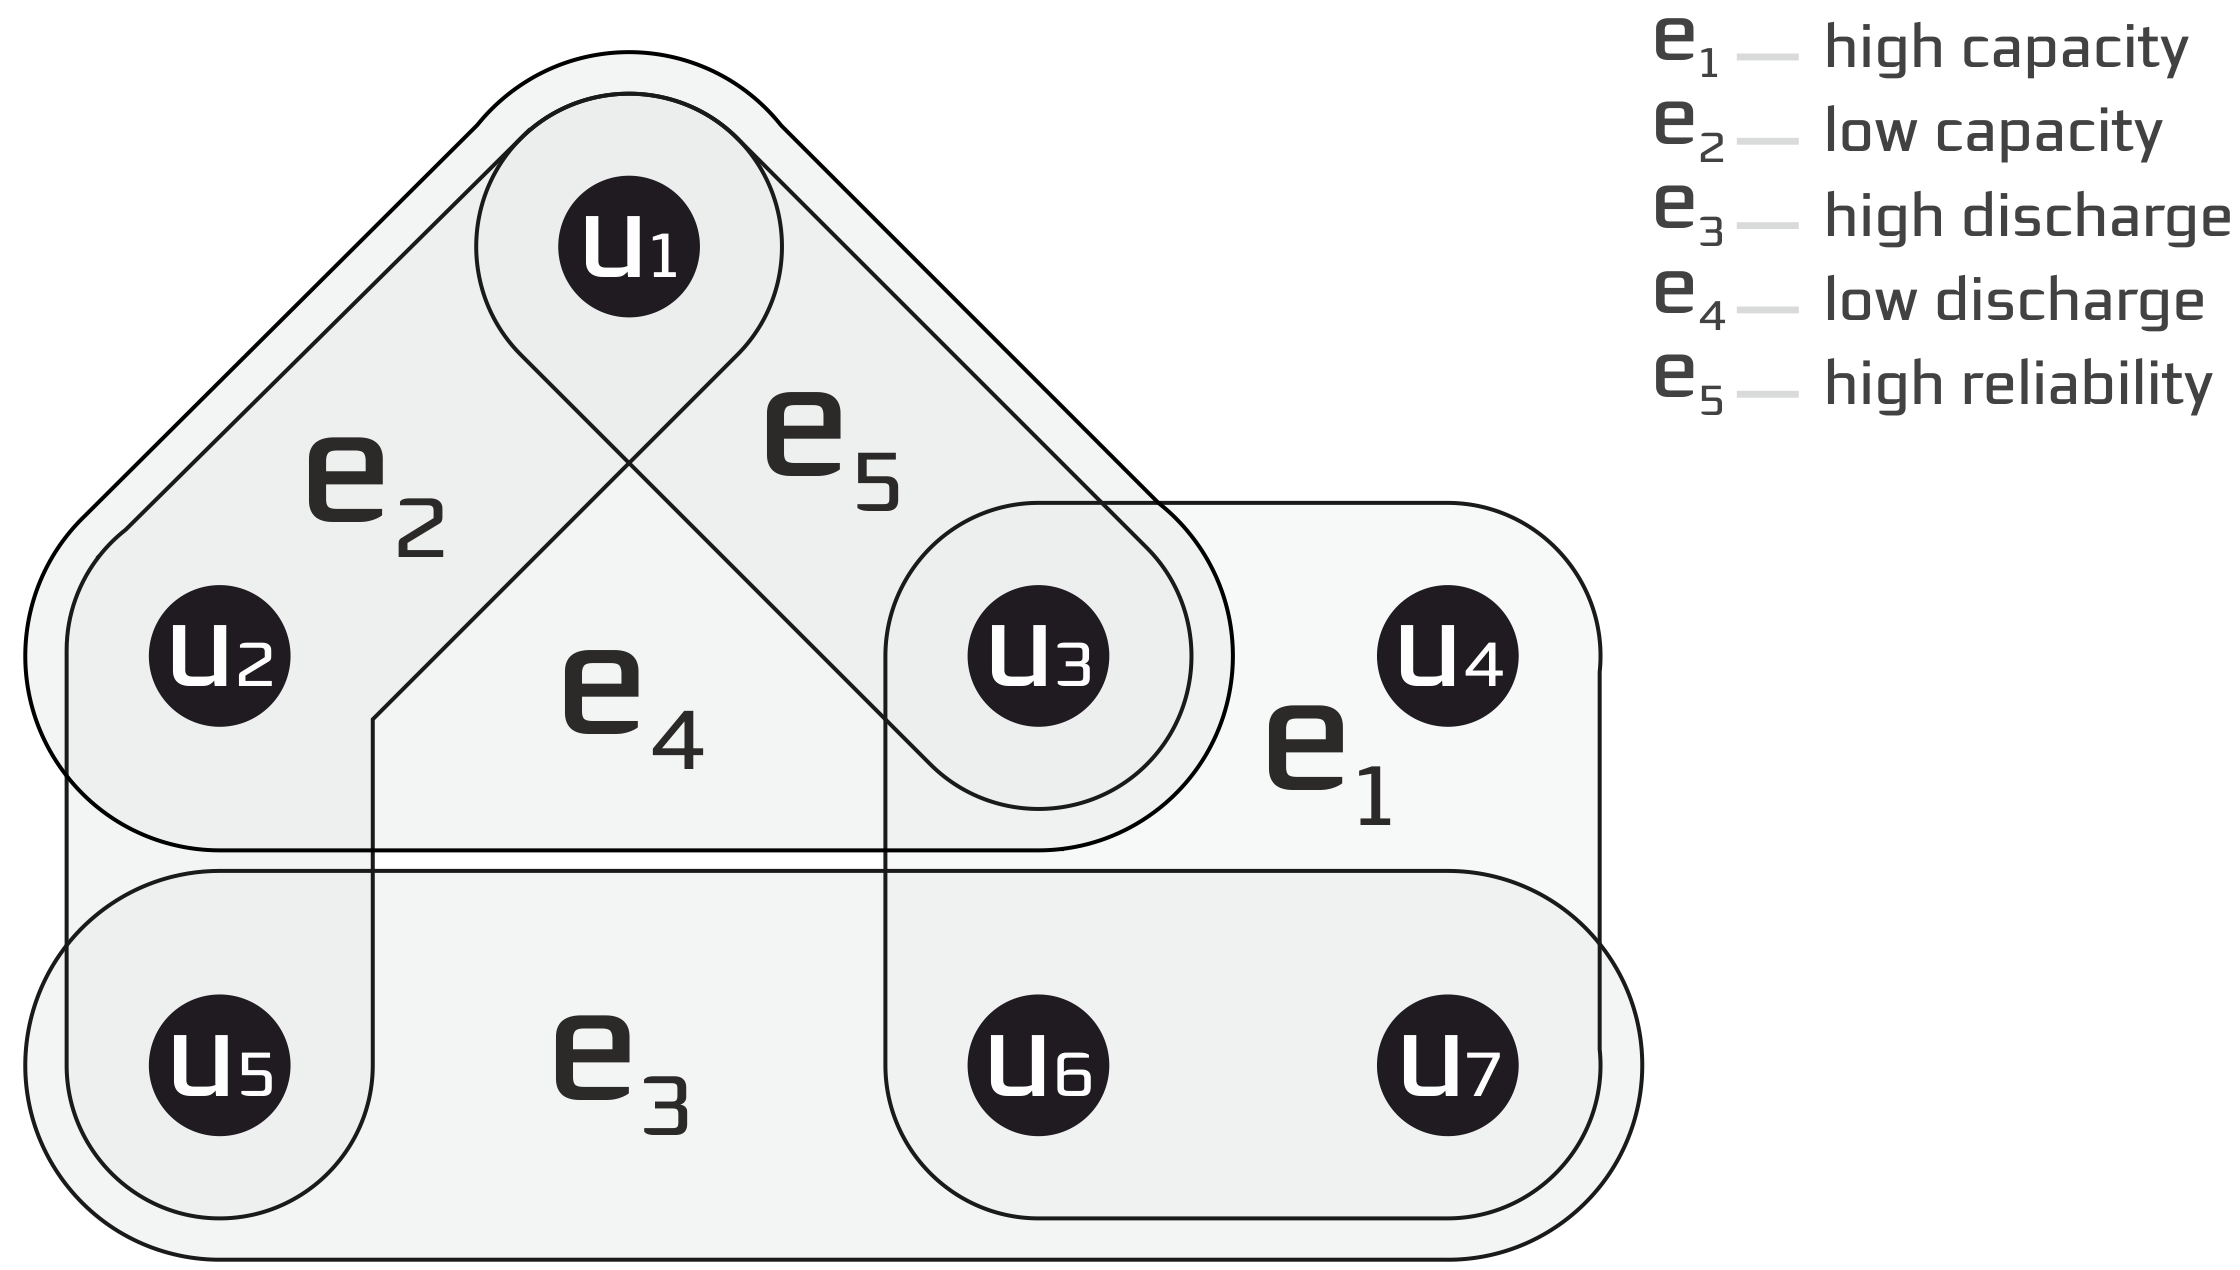
\includegraphics[scale=0.3]{hypergraph.png}
		\caption{A simple hypergraph\label{fig:hypergraph}}
	\end{minipage}%
	\begin{minipage}{.5\textwidth}
		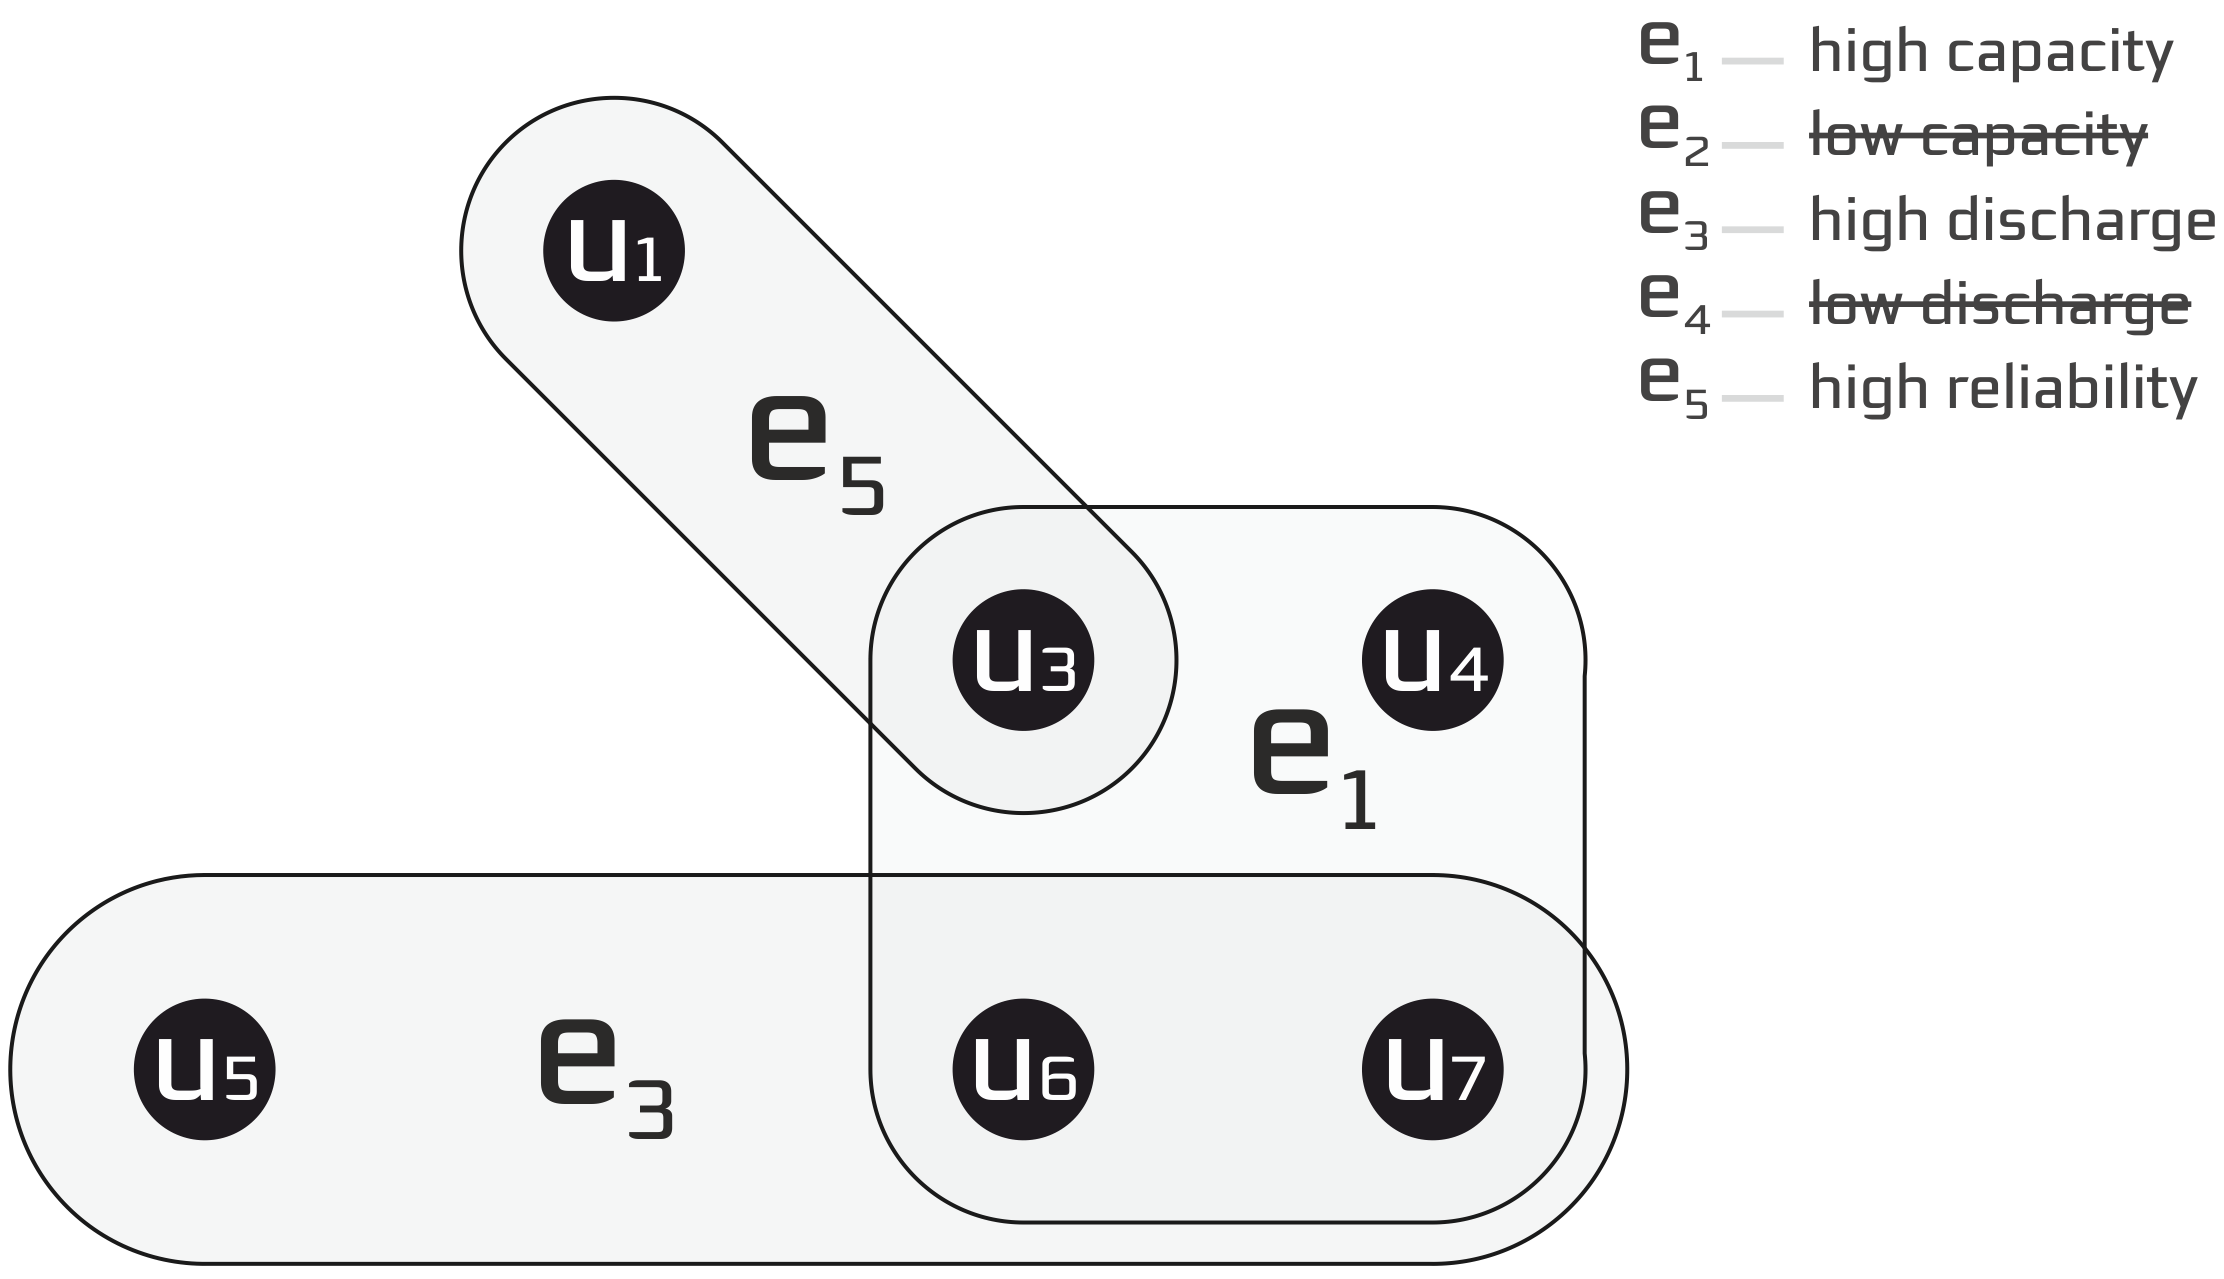
\includegraphics[scale=0.3]{hypergraph_prune.png}
		\caption{Pruning a simple hypergraph\label{fig:hypergraph_prune}}
	\end{minipage}
\end{figure}

In order to develop multi-criteria coalition formation algorithms that generate coalitions efficiently, we employ the concept of {\em a hypergraph}.
A hypergraph $H = (V, E)$ is a generalization of a graph, where each {\em hyperedge} $e \in E$ can contain any number of {\em vertices (or nodes)} in the set $V$.
Vertices in $H$ correspond to agents; while we view a hyperedge as corresponding to some particular {\em attribute} or {\em characteristic} possessed by the agents in the hyperedge.
In the V2G setting, the agents correspond to EVs (i.e., an EV is represented by a node in our hypergraph); while the hyperedges correspond to vehicle characteristics. More specifically, a hyperedge corresponds to a ``quality level'' of some EV attribute, as we explain below.

In order to represent the different {\em quality} of the various hyperedges, and utilize it in our algorithms, we mark each hyperedge with a weight.\footnote{In our implementation, the weight of the edges, according to the quality of each attribute(capacity, reliability and discharge), are as follows: \{\textit{extremely-high: 8, very-high: 7, high: 6, medium-high: 5, medium-low: 4, low: 3,very-low: 2, extremely-low:1}\}. Thus we have 24 edges + 1 containing commitment of EVs.} These weights define the \textit{degree} of a node: {\em The degree $deg(u)$ 
	of a node 
	$u$ 
	is the sum of the weights of its edges}. Intuitively, {\em a high degree node is a high quality one}. This fact is exploited in our algorithms below.
A hyperedge (of a given quality) will be also called a {\em category}. The (quality of the) categories to which an EV belongs will be influencing the decisions of our {\em hypergraph pruning} algorithm, which we describe in Section~\ref{sec:pruning} below. A node that belongs to a hyperedge characterizing the quality of a given agent attribute, cannot belong to some other hyperedge characterizing the quality of the same attribute.


To illustrate the use of hypergraphs in our setting, consider for example the hypergraph of Fig.~\ref{fig:hypergraph}, which contains the hyperedges $e_{1...6}$ and vertices $u_{1...7}$. It is clear in this example that vertices may belong to multiple hyperedges: the hyperedge $e_1$ contains the vertices $u_{3,4,6,7}$, while the vertex $u_1$ belongs in the hyperedges $e_2, e_5, e_4$. Vertices in Fig.~\ref{fig:hypergraph} correspond to EVs; while the hyperedges correspond to the ``quality'' of the following EV attributes: \textit{capacity}, {\em discharge rate} and \textit{observed reliability}. The meaning of these attributes is intuitively straightforward, but will be nevertheless explained in Section~\ref{subsec:criteria} below. Each attribute is related to at least one hyperedge in the hypergraph. For instance, in Fig.~\ref{fig:hypergraph}, the {\em capacity} attribute is represented by three hyperedges in the hypergraph: {\em low-capacity}, {\em medium-capacity}, and {\em high-capacity}. As noted above, no node can belong in more than one capacity-related hyperedges. In our figure, 
\begin{itemize}
	\item the hyperedge $e1$ represents the nodes which have high capacity;
	\item the hyperedge $e2$ contains nodes that have low capacity;
	\item $e3$ and $e4$ include the vehicles with high and low discharge rate, respectively;
	\item finally, $e5$ contains nodes that are expected to the {\em highly reliable}.
\end{itemize}
For example, node $u1$ is a {\em low-capacity}, {\em low-discharge} but {\em highly reliable} vehicle---while node $u3$ is a {\em high-capacity}, {\em low-discharge} and {\em highly reliable} one.

%       A simplified example of how we store attributes of a hypergraph is presented in Figure~\ref{fig:hypergraph}.

%       If we were to simplify our hypergraph to the size of the example, then Figure~\ref{fig:hypergraph} would be our hypergraph with seven nodes $u \in V$ and five hyperedges
% $e \in E$. These nodes would represent vehicles and each hyperedge represents a specific attribute as we can see in the legend.

%       It should be noted that in the hypergraph we used in our experiments, there were several more hyperedges.

Organizing the information relating to specific agent attributes using hyperedges, enables us to both access this information efficiently, and keep it organized.
Moreover, in many settings, agent characteristics captured by hyperedges, naturally correspond to criteria according to which we can form coalitions.
For example, it is conceivable that we want to use agents with {\em high capacity} from the respective {\em high-capacity} edge, if our goal is to form coalitions with {\em high capacity}. Our approach of using hypergraphs is even more generic than what implied so far, since we can easily define hyperedges that contain agents which are or are not {\em permitted} to connect with each other, for various reasons; and since we can exploit the hypergraph to allow the formation of coalitions according to a multitude of criteria.

\subsection{Criteria for Forming Coalitions}
\label{subsec:criteria}

The algorithms presented in this work can be employed by any entity or enterprice (such as the Grid, utility companies or Smart Grid cooperatives) that wants to form EV coalitions for the V2G problem, using any set of criteria of its choosing. Here we identify three such natural criteria, namely \textit{reliability, capacity} and \textit{discharge rate}. These formation criteria are consistently mentioned in the related literature, though perhaps not with these exact names, and not explicitly identified as such~\cite{kamboj2010exploring,kamboj2011deploying,valogianni2014effective}.

First of all, a coalition has to be consistently {\em reliable}, i.e. it should be able to serve the power that has been requested without any disruptions. For a coalition to be reliable, its members must be reliable too, and gaps in reliability must be met with backup agents. We define {\em agent reliability} as {\em the estimated probability that an agent will fulfill its promises}. The {\em promise} of an agent is its {\em commitment} on being connected to the Grid during a specific time slot in order to contribute via providing energy to the Grid, if so requested. Such slots naturally correspond to electricity trading intervals.

%Since the coalitions are formed to offer power services in future time slots, agents can be asked to state their availability.
%This availability is stored in commitment hyperedge .

In addition, a coalition must fulfill a {\em capacity} requirement. 
The {\em capacity} of a coalition is the amount of electricity (measured in $kWh$) the coalition will be offering to the Grid; 
while the capacity of en EV is, similarly, the amount of electricity (in $kWh$) the EV will be offering to the Grid.
In fact, gathering enough EV capacity to cover the Grid needs during high demand periods, is the main objective of any V2G solution. 
%Naturally, creating a coalition to meet a high power peak requires a considerable amount of capacity offered. 
%On the other hand minor peaks can be stabilised by building EV coalitions with a much lower capacity.

Another factor in the V2G problem is the {\em discharge rate} of a coalition (or, of a single EV)---the rate by which the coalition (resp., the EV) is able to provide (electrical) energy to the Grid over a specified time period. Discharge rate is measured in $kW.$ % (=$kWh / h$).
A high coalitional discharge rate could be required in cases where capacity should be offered within a small amount of time, for example when the Grid is under a heavy demand load. 
Naturally, a coalition has a high discharge rate if its members discharge rates are high; for our purposes, we assume that the discharge rate is additive, i.e., the discharge rate of a coalition is the sum of its EVs discharge rates.
In Section~\ref{sec:results}, we will be forming coalitions in order to meet specific capacity and discharge rate targets; and observing how reliable the coalitions meeting these targets are.

Now, the hypergraph used in our current implementation was designed so that it could easily satisfy requests pertaining to these particular criteria.
As such, there was a total of $25$ hyperedges in the hypegraph---\{{\em extremely-high, very-high, high, medium-high, medium-low, low, very-low, extremely-low}\} $\times$ \{{\em capacity, discharge rate, reliability}\}; and a {\em committed} one, containing EVs that have stated they will be connecting to the Grid during the particular slot.%\footnote{We could have stored the commitment of the EVs on a ``per time slot'' basis, by using several hyperedges (one per slot) without any additional cost. However, in our experiments, we focus on a single time slot only.}

In our model, we assume that, at any time step that this is required---due to a consumption peak, an unplanned event, or the need to regulate frequency and voltage---the Grid (or some other entity) advertises its demand for a V2G coalition with several desirable characteristics. As noted in~\cite{kamboj2011deploying}, individual EVs are well-suited for providing services at short notice. What we show in this paper, is that we can select agents from a huge pool of EVs to form {\em coalitions} that are able to provide large amounts of power at short notice, and with high reliability.


%To effectively extract nodes from the hypergraph we put forward the following three methods.
%\begin{itemize}
%	\item {Minimal Transversal} \cite{kavvadias2005efficient}
%		\item {Clustering} \cite{zhou2006learning}
%		\item {Heuristic Approach}
%	\end{itemize}
%	Preceding the above approaches, though, we have noticed that pruning the hypergraph to include EVs only from the hyperedge we are interested in, is extremely efficient. For example, we always prune the hypergraph to keep nodes from the "Committed" hyperedge, and we also prune the hyperedges that signify low values of an attribute.


\subsection{Pruning the Hypergraph}\label{sec:pruning}

An important aspect of using hypergraphs for dealing with large state-spaces, is the resulting ability to perform node and edge pruning. Since dozens or hundreds of thousands of our EVs populate the hypergraph, and each one is a member of several hyperedges, running the algorithms without pruning would require an enormous amount of computing power. However, due to the nature of the hypergraph, and the way we store our vehicles and their attributes, it is extremely easy and effective to narrow down the number of vehicles and edges used, by leaving out EVs that are less promising as coalition members. For example, if achieving a high capacity for the to-be-formed coalition is a key goal, then, intuitively, we can narrow down our search for coalition members by focusing only on nodes belonging to the set of hyperedges (or ``categories'') $high capacity \cup very high capacity \cup ex high capacity$. 

% We use this method in all our algorithms with small modifications to each one, in order to relieve bottlenecks.	
To illustrate pruning, Fig.~\ref{fig:hypergraph} shows a hypergraph that contains all EVs. In order to reduce the size of the hypergraph and thus the computing requirements, we could keep only EVs belonging to at least one high quality edge, as shown in Fig.~\ref{fig:hypergraph_prune}. 


\begin{algorithm}
	\caption{Pruning the Hypergraph}\label{alg:pruning}
	\begin{algorithmic}[1]
		\Procedure{Pruning}{$H$, $CategoriesKept$}
		\For{Hyperedge $\in$ H}
		\If{$Hyperedge \in CategoriesKept\cap Committed$}
		\State $NewHEdges\gets NewHEdges \cup HyperEdge$
		\State $NewNodes\gets NewNodes \cup HyperEdge.nodes$
		\EndIf
		\EndFor
		\State $NewHGraph \gets Hypergraph(NewNodes, NewHEdges)$
		\EndProcedure
	\end{algorithmic}
\end{algorithm}

Algorithm~\ref{alg:pruning} is our implementation of pruning. The algorithm iterates over all hyperedges in the given hypergraph $H$, and 
keeps only the nodes belonging to hyperedges that correspond to the specified ``categories of interest'' ({\em CategoriesKept} in Alg.~\ref{alg:pruning}).

In our implementation, the {\em CategoriesKept} are heuristically selected, and depend on the algorithms. For instance, the {\em minimal transversal} algorithm requires a more aggressive pruning, since its complexity is sensitive to the number of nodes used as input (cf. Section~\ref{sec:transversal}), and we therefore empirically feed it with as few hyperedges as possible. 
%In section~\ref{sec:generating} we provide ~\ref{tab:pruningres} showing the efficiency of our pruning algorithm.

Our experimentation indicates that the use of pruning can lead to a significantly smaller hypergraph, and to vast improvements in terms of execution time for our algorithms.  In our simulations, the hypergraphs are pruned to about $1/20$ of the initial size of the EVs pool, without sacrificing the methods' performance (cf. Section~\ref{sec:generating}). Moreover, pruning using Algorithm~\ref{alg:pruning} is almost instantaneous.

\subsection{Minimal Transversal Algorithm} \label{sec:transversal}
Using hypergraphs allows to use an intuitive approach  for locating agents for coalitions: to generate the set of \textit{minimal transversals} for the \textit{high-value hyperedges}~\cite{eiter1995identifying}. A \textit{transversal} (or \textit{hitting set}) of a hypergraph H, is a set $T\subseteq V$ with hyperedges $X$ where $X = E$ (i.e., vertices in $T$ belong to \textit{all} hyperedges in $E$). A \textit{minimal transversal} is a set that does not contain a subset that is a hitting set of $H$.  As such\footnote{Of course there can be more than one minimal transversals, and it is not necessary that they have the same cardinality.}, generating several minimal transversal sets for \textit{high-quality} hyperedges is expected to identify agents which are high-quality and should be used in the formation of a coalition. Subsequently, we join those agents together until our criteria are met. 

Our approach with the minimal transversal set is to prune all edges but those of extremely high quality that are also ``committed'', as seen in Algorithm~\ref{alg:transversal}. Then we generate progressively the minimal hitting sets, using an algorithm similar to \cite{eiter1995identifying}. That is, we first generate the minimal hitting sets containing one node, then those with two, and so on. Then we randomly pick agents belonging to those minimal transversals, until the coalitions requirements are met. If the requirements are met during the progressive minimal transversal generation process, no further minimal transversals are generated.

To illustrate this concept with the help of Fig.~\ref{fig:hypergraph}, we prune the hypergraph to keep only the high-quality edges $e_1, e_3, e_5$, leaving us with the nodes $u_1, u_3...u_7$ and edges $e_1, e_3, e_4$, as seen in Fig.~\ref{fig:hypergraph_prune}. Then we generate all the minimal transversal sets. The minimal transversals generated first are the ones with two nodes (since there are no minimal transversals with one node) i.e. the following$\{u_3, u_5\}, \{u_1,u_7\}, \{ u_6, u_1\}$.%,\newline$\{ u_3, u_7\},\{ u_3, u_6\} $.

This method creates a set of agents with uniformly distributed high-quality characteristics. Though this is desirable in theory, in practice the results vary depending on the generated minimal transversal set. There are characteristics which might be of higher importance than others and this cannot be taken into account by the transversal algorithm due to its nature. Regardless, this method could be of much use for creating a base of quality agents; for uniformly improving the quality of an already formed coalition by adding agents from the minimal transversal sets; and for creating versatile coalitions without focusing on specific attributes.

\begin{algorithm}
	\caption{Coalition formation using Minimal Transversal}\label{alg:transversal}
	\begin{algorithmic}[1]
		\Procedure{MinimalTransversal}{$H$}
		\State $H \gets Prune(H, exhigh)$ \Comment exhigh signifies all hyperedges with exhigh qualities
		\State $T= \emptyset$, $C = \emptyset$ \Comment Start with an empty coalition
		\For{i=1 to $|E|$} \Comment where $|E|$ is the number of edges in the (pruned) $H$
		\State Create the union $U$ of minimal transversal sets with size $i$, generated from $H$.
		\State $T$ = $T$ $\cup$ $U$
		\While{$C$ does not meet the criteria}
		\State Randomly select an {\em unselected} node  $\in T $ and add it to $C$
		\EndWhile
		\If{criteria have been met}
		\State return formed coalition $C$
		\EndIf
		\EndFor
		\EndProcedure
	\end{algorithmic}
\end{algorithm}

Line 6 of Algorithm~\ref{alg:transversal} is our implementation of minimal transversal~\cite{eiter1995identifying}. Though there is no known polynomial time algorithm for the general hypergraph transversal problem, the algorithm given was shown experimentally to behave well in practice, and its memory requirements are polynomially bounded by the size of the input hypergraph, though it comes without bounds to its running time.

\subsection{Clustering Algorithm}\label{sec:Clustering}
The second approach is to create clusters of agents. After creating said clusters, we efficiently calculate the best cluster and then sample EVs from that group until our coalition criteria are met.

In more detail, we first generate a hypergraph of EV agents with the characteristics described previously. Then, hypergraph clustering is performed.
The hypergraph clustering itself is an implementation of that proposed in \cite{zhou2006learning}, and is conducted as follows. 	%On the hypergraph we have generated we also add weights in the hyperedges. 
%The weights correspond on the label (high, medium, low) of the attribute and are going to be used later for locating high valued agents.

We begin by implementing functions that calculate
\begin{itemize}
	\item{\em the Incidence Matrix}: A %$|V|\times|E|$%
	matrix $H$ with entries $h(u,e) = 1$ if $u \in e$ and $0$ otherwise.
	\item{\em the Weight Matrix}: A diagonal matrix $W$ containing the weights of the hyperedges.
	\item{\em $D_u$ and $D_e$}: Matrices containing the node and hyperedge degrees respectively.
	\item{\em the Adjacency Matrix}: A matrix defined as $A = HWH^T - D_u$
\end{itemize}
The matrices above are used for the final calculations of the hypergraph \textit{Laplacian matrix}. This a matrix representation of a graph, that has information on the degrees of the nodes, and their connections with the hyperedges (cf.~\cite{zhou2006learning}, Section 5). 
%After its calculation, the Laplacian contains the node degrees in its diagonal (which enables us to discard the $D_u$ matrix, for memory efficiency).

As explained in~\cite{zhou2006learning}, having the Laplacian, enables us to calculate the $\Phi$ eigenvectors $[\Phi_1 ... \Phi_k]$ corresponding to the $k$ lowest eigenvalues. These can then define $X = [\Phi_1 ... \Phi_k]$, a matrix that can be employed for $k$-way partitioning to cluster our agents. This is achieved via running the $k$-{\em means} algorithm \cite{hartigan1979algorithm} on the row vectors of $X$\cite{zhou2006learning}. As explained in \cite{zhou2006learning}, the rows of X are representations of the hypergraph vertices in the $k$-dimensional Euclidean space. Of course, choosing a value for $k$ has to be decided empirically. In Section~\ref{sec:results_modifications} we will be testing different values for $k$. 
After generating the clusters, we are given the task to locate the ``best'' cluster among them. To do this efficiently, we simply sort them by looking at {\em the average of the node degrees}.
%\footnote{Note that the Laplacian matrix can also be used to extract easily high-quality agents, by retrieving nodes that have high values (high node degrees) in its diagonal.}
This provides us with a cluster that is better than the rest. We then sample nodes from the best cluster until our criteria are met. Algorithm~\ref{alg:clustering} summarizes the method.

\begin{algorithm}
	\caption{Coalition formation using Hypergraph Clustering}\label{alg:clustering}
	\begin{algorithmic}[1]
		\Procedure{Clustering}{$H$}
		\State $H \gets Prune(H, (vhigh \cup exhigh))$ \Comment exhigh and vhigh signify the sets of extremely high and very high quality hyperedges respectively
		\State Generate k clusters using the algorithm described in~\ref{sec:Clustering}~\cite{zhou2006learning}
		\State $C = \emptyset$ \Comment Start with an empty coalition
		\State Find the best cluster, $A$, by comparing the sum of node degrees of each cluster.
		\While{$C$ does not meet the criteria}
		\State Randomly select a node $\in A $ and add it in $C$
		\EndWhile        
		
		\EndProcedure
	\end{algorithmic}
\end{algorithm}

\subsection{A Heuristic Algorithm} \label{sec:heuristic}
While using a minimal transversal generates quality sets of agents, computing the {\em degree} of a node can identify single agents with many quality attributes. As an example, when we have a reliable coalition as a base but we require more capacity, we can use the sorted list we have generated, to pick agents with high capacity. Intuitively, this approach will result to picking high overall quality agents for our coalition. We can also create coalitions by using only the best available agents. Moreover, we can use the aforementioned sorted-by-degree list of nodes in order to "fill gaps" and improve on the quality of already formed coalitions. 

Thus, our heuristic method operates as follows. {\em (1)} First, we prune the hypergraph to include only ``promising'' nodes and hyperedges. For instance, we exclude nodes not in {\em extremely high} or in {\em very high} hyperedges. {\em (2)} Then we sort the remaining nodes based on their node degree. {\em (3)}  Finally, we pick the highest degree nodes from the list until the coalition criteria are met. By starting at the top of the list, we can guarantee that agents have many positive characteristics. 

We can see at step {\em (1)} above, that this algorithm, like the rest of our methods, employs pruning. As such, it does exploit the hypergraph structure. However, in practice the algorithm can deliver excellent results without much pruning. In our experiments in Section~\ref{sec:results} below, the heuristic approach is shown to outperform the rest while pruning only the non-committed nodes in the hypergraph. In fact, one strength of this approach is that it does not {\em rely} on pruning, since its complexity is low: essentially, that of the algorithm employed for sorting (i.e., $O(nlogn)$, since we use with Python's built-in {\em Timsort} algorithm). By not relying on pruning, the algorithm can focus on promising nodes with high node degree (and, therefore, quality), irrespective of the exact hyperedges to which they belong.

\subsection{A Simple Sampling Method}
For interest, and in order to have a benchmark for the rest of our algorithms, a simple sampling algorithm was also developed. The algorithm takes random samples until the specified goals are achieved.
%We will implement the methods above and compare the results.
% Chapter 1

\chapter{Chapter Title Here} % Main chapter title

\label{Chapter1} % For referencing the chapter elsewhere, use \ref{Chapter1} 

%----------------------------------------------------------------------------------------

% Define some commands to keep the formatting separated from the content 


%----------------------------------------------------------------------------------------



\section{Experiments and Results}\label{sec:results}

In this section we present the evaluation of our algorithms. First we explain how the EV population is generated, and the time this generation process takes. Then, the performance of the algorithm is evaluated in terms of the quality of the formed coalition and also in terms of execution time and scaling behavior. All figures and tables present average values over multiple runs. Specifically, we generated $20$ hypergraphs  with $20,000$ EVs each, and then ran each algorithm on every hypergraph 10 times, and took the averages (and the average of those averages).
%First, we will see the time required to generate the pool of EVs we will be using in our tests. Next, we will present how each algorithm performed while it was running and when the coalitions were in the process of being formed. We will also test small modifications to our algorithms. Finally, we present graphs of how our algorithms scale with population and goals. 
%\subsection{A Note on Computational Requirements}
%Generation of the graph is $O(n)$. Each insertion is $O(1)$. For the minimal transversal algorithm the complexity as calculated in \cite{kavvadias2005efficient} is $O(\log^2 n)$. That's for calculating all the minimal transversal sets. For the heuristic approach, normal sorting complexity is applied on the pruned hypergraph.
Our experiments were run on a Sandy Bridge i7-2600K at 4.2 GHz. All the tests were running on a single thread on Python, meaning that there is a lot of room for optimization. %To generate the graphs below 20 sets of starting EVs were made for each pool size and the algorithms run ten times in each one. This was done to balance out the timing errors %that could be introduced from the different set of EVs. 

\subsection{Generating the EV Population}\label{sec:generating}
To generate the population for each type of experiment we create the vehicles one by one, by first generating its properties as follows. The capacity of each vehicle is generated from a Gaussian distribution with mean value $100$ and $\sigma = 80$. The discharge rate of each vehicle is generated from a Gaussian distribution with mean value $10$ and $\sigma=5$. The reliability of each vehicle is picked from a Gaussian distribution with mean value $0$ and $\sigma=1$. Each EV's commitment of being connected to the Grid is a {\em true} / {\em false} variable, with a $0.9$ probability of being {\em true}. If {\em true}, then the EV is inserted in the {\em committed} hyperedge. When a vehicle has its properties created, it is added in the pool of available EVs. The computational complexity of generating the hypergraph is, as expected, $O(n)$.

The coalition requirements are set to values which are commonly used in the regulation market \cite{kamboj2011deploying}, namely the following two. First, each coalition must have a total capacity of at least $10MWh$. The discharge rate must also be at least $1MW$ \cite{kamboj2011deploying}
These values are kept constant throughout all experiments---except when we test scaling against an increasing capacity goal, where capacity is treated as a variable.
%\footnote{As stated in Section~\ref{sec:approach}, our hypergraph used 25 hyperedges to store the attributes.}


%\begin{figure}\centering
%	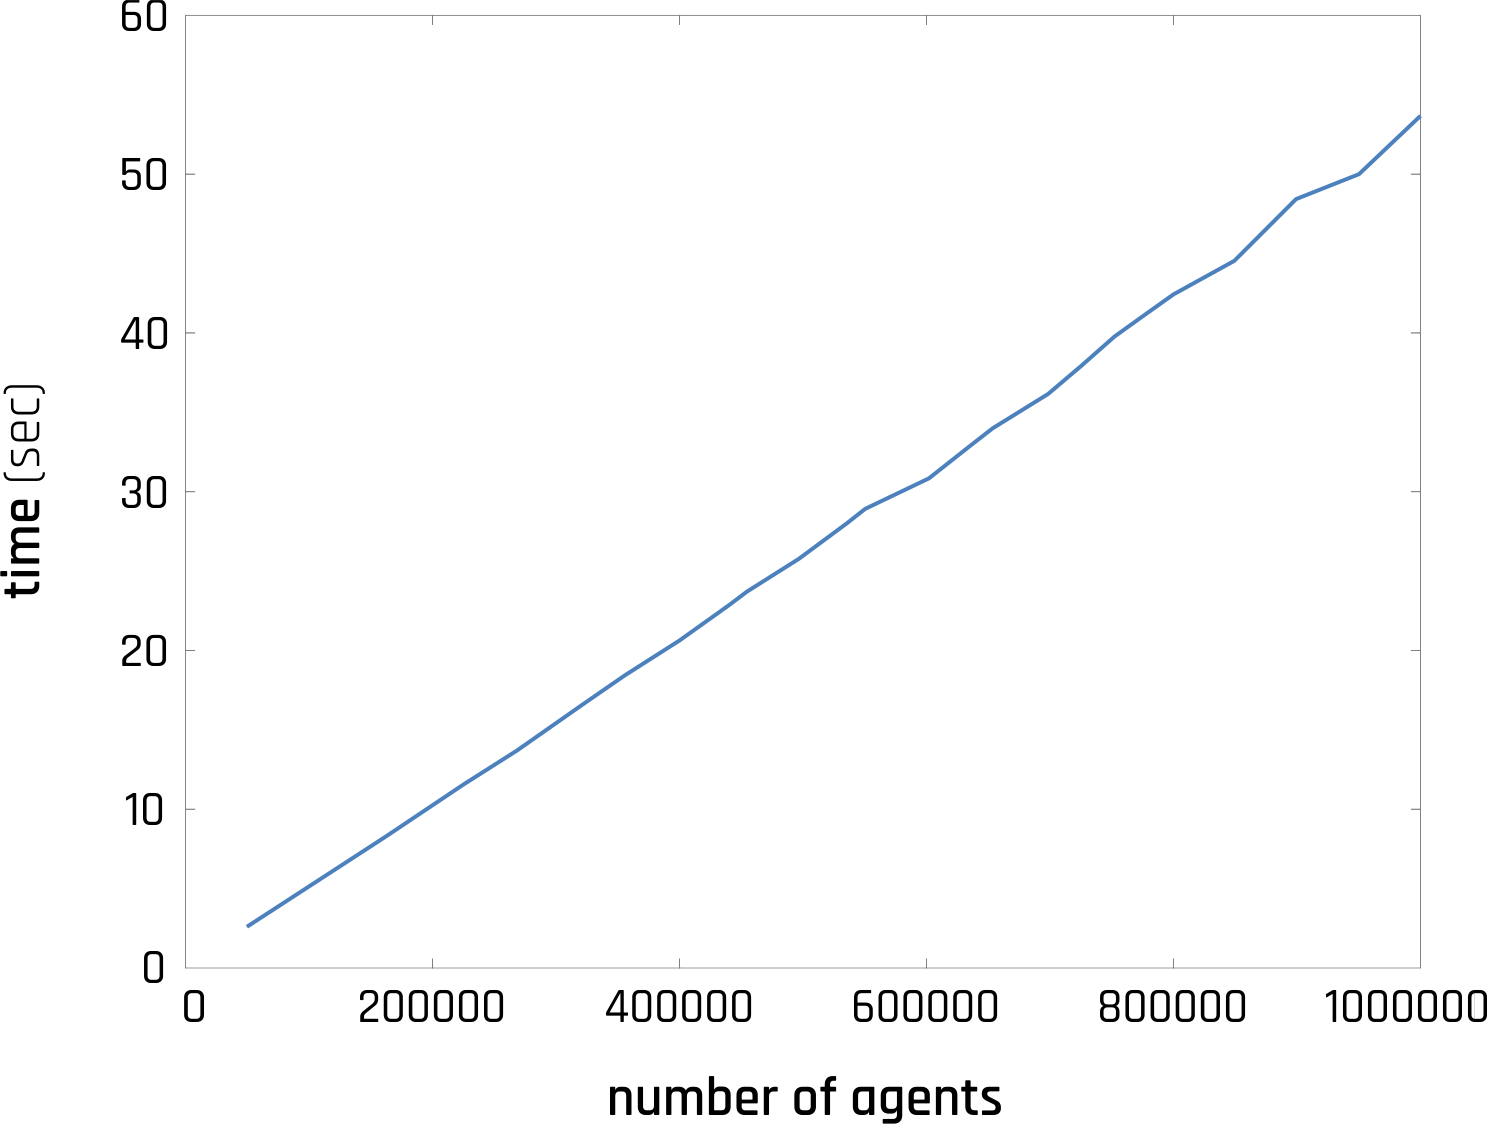
\includegraphics[scale=0.3]{generation_scaling.png}
%	\caption{Hypergraph generation scaling\label{fig:genscaling}}
%\end{figure}
Creating the hypergraph is a problem that scales linearly with time. Specifically, generating the hypergraph, including the vehicles and distributing them to hyperedges, takes a very small amount of time and scales linearly up to a million within a minute (Table ~\ref{tab:resultssum}).
%	\begin{table}
%		\begin{center}
%			\begin{tabular}{| c || c | }
%				\hline
%				EVs & Generation Time (sec) \\ \hline
%				100,000  & 5.08\\ \hline
%				200,000  & 10.23 \\ \hline
%				300,000  & 15.31  \\ \hline
%				400,000 & 20.51  \\ \hline
%				500,000 & 25.75   \\ \hline
%				600,000 & 30.69   \\ \hline
%				700,000 & 36.14   \\ \hline
%				800,000 & 42.38   \\ \hline
%				900,000 & 48.37   \\ \hline
%				1,000,000 & 53.62   \\ \hline
%			\end{tabular}
%		\end{center}    
%		\caption{Hypergraph generation scaling timings\label{tab:genscaling}}
%	\end{table}
\begin{table}
	\begin{center}
		\begin{tabular}{| c || c | c | }
			\hline
			Algorithm & Nodes after Pruning & Edges after Pruning \\ \hline
			Transversal & 1148.4   & 4  \\ \hline
			Clustering  & 1218.8   & 7 \\ \hline
			Heuristic   & 18012.6  & 25 \\ \hline
		\end{tabular}
	\end{center} 
	\caption{Pruning Results\label{tab:pruningres}}
\end{table}
As mentioned above, the initial EV population was $20,000$ nodes. However, before feeding the nodes to the algorithms, we pruned the hypergraph to keep promising nodes. Table~\ref{tab:pruningres} shows the average hypergraph size finally fed to the algorithms.

\subsection{Forming the Coalitions}
We now proceed to evaluate the performance of our algorithms. Our evaluation will examine {\em (a)} how fast and {\em (b)} by selecting how many vehicles they can meet the set requirements. Naturally, the faster an algorithm forms a coalition that meets all the requirements, the better. 
\begin{figure}
	\centering
	\begin{minipage}{.5\textwidth}
		\centering
		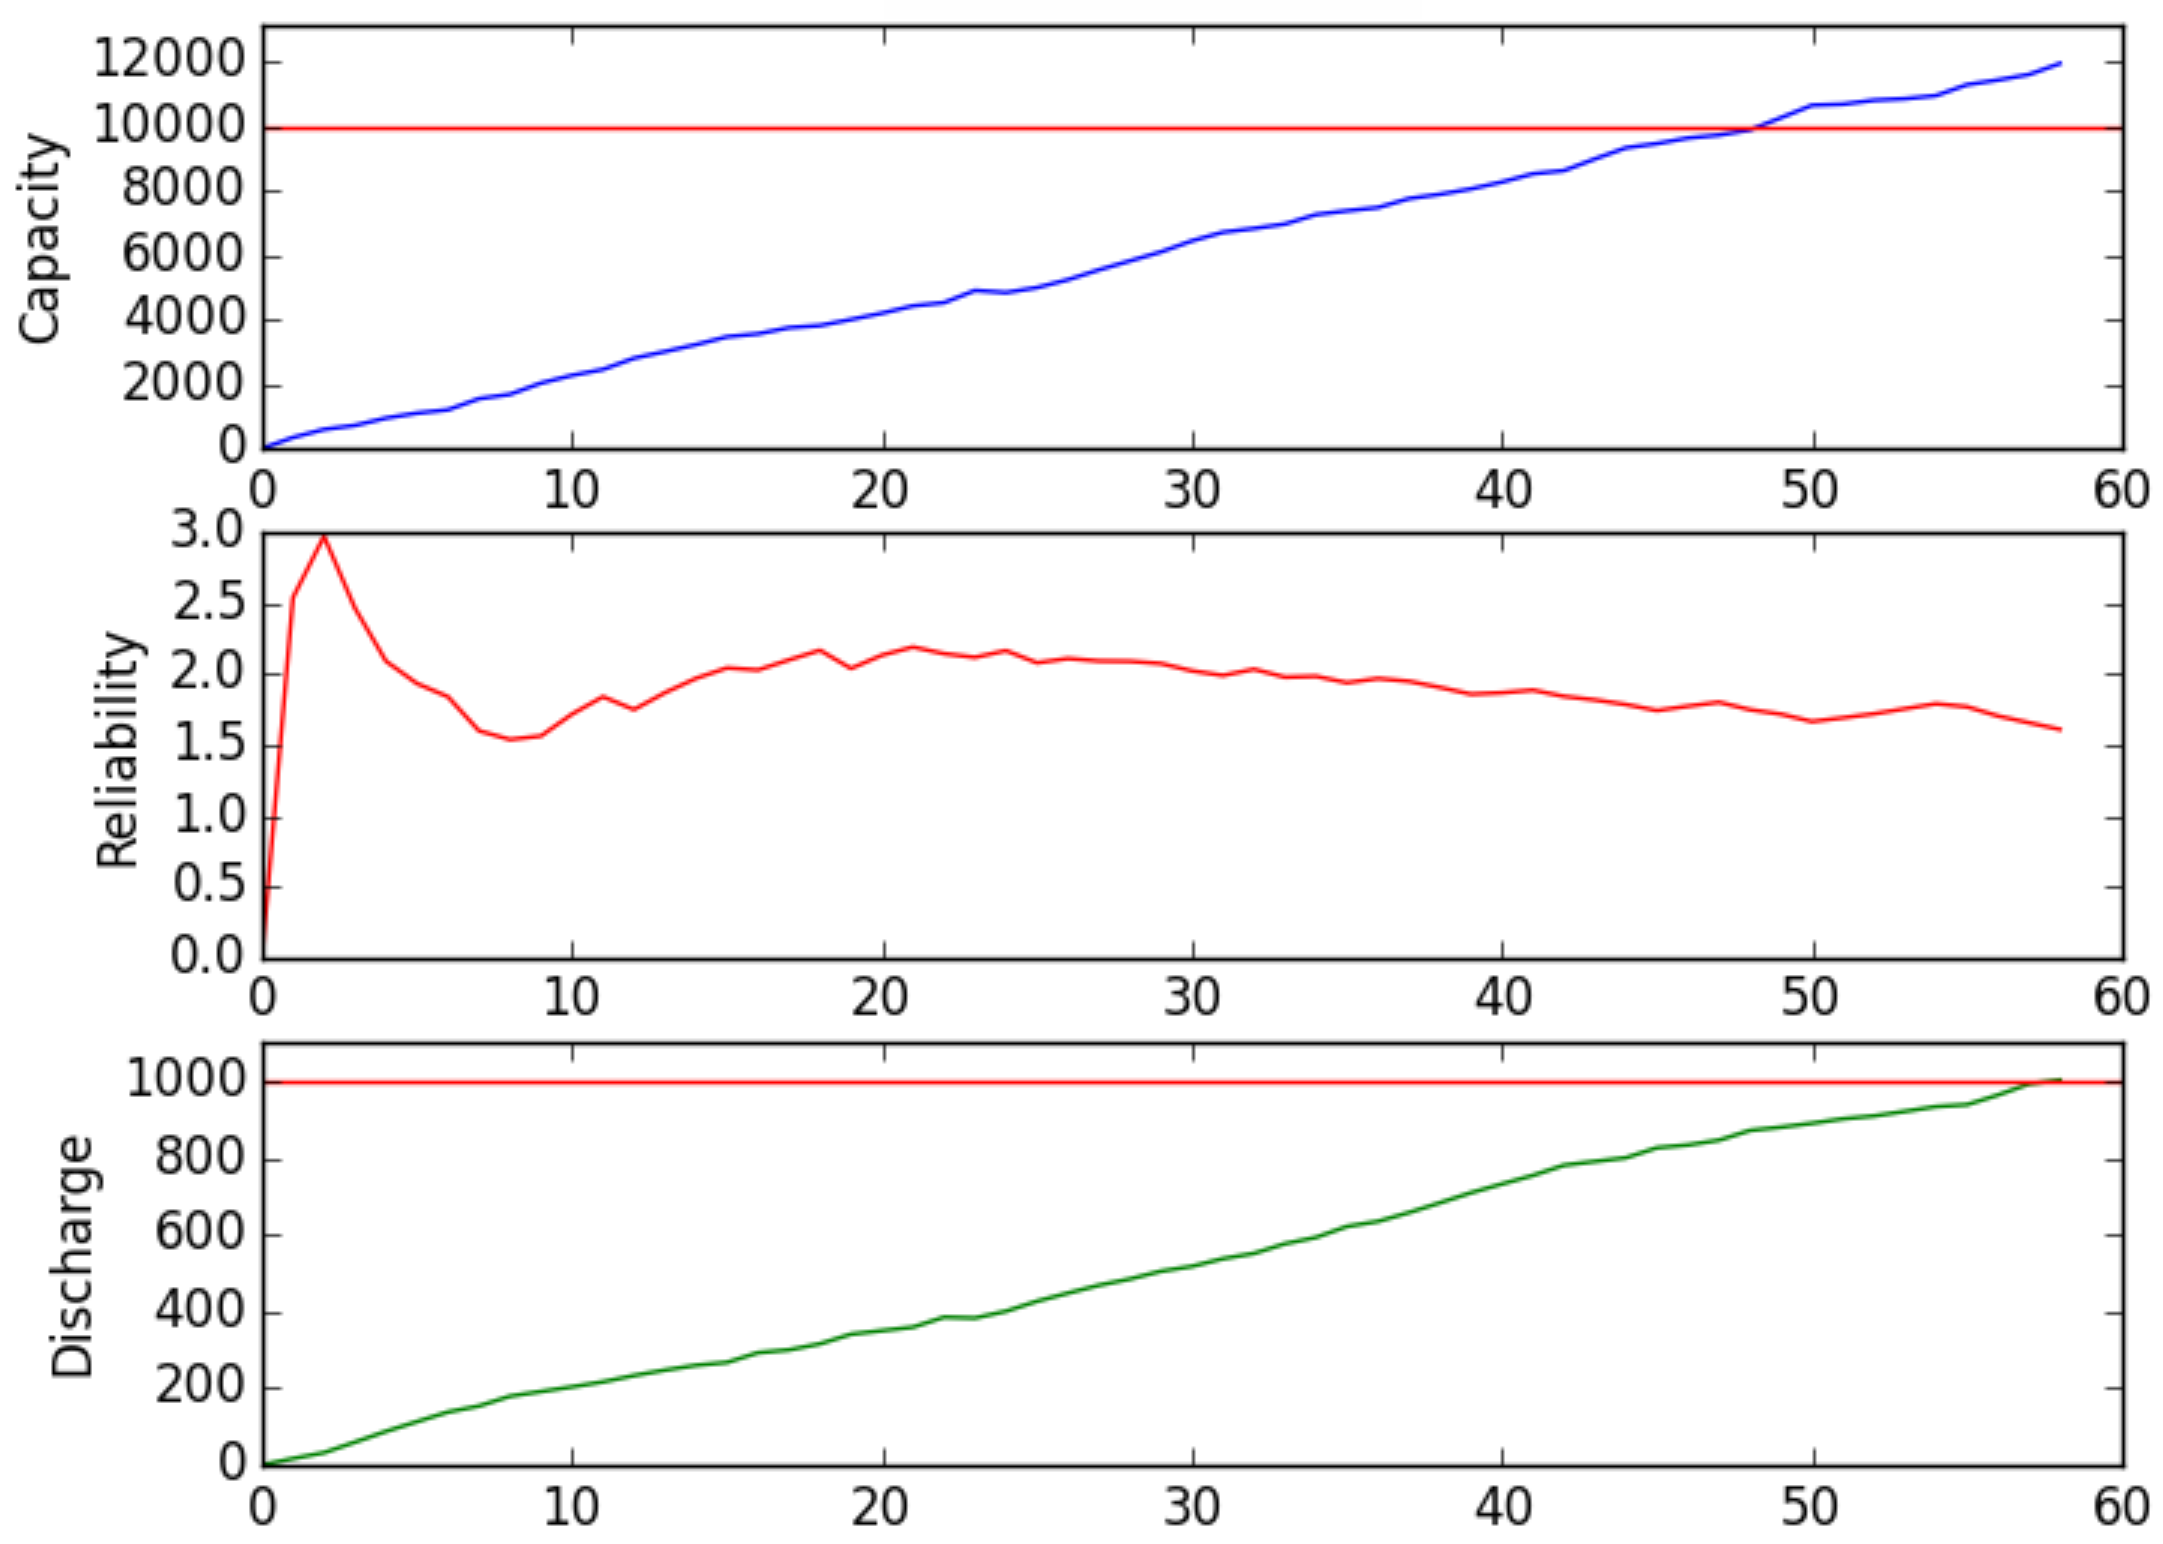
\includegraphics[scale=0.3]{greedy.png}
		\caption{Coalition formation with the\newline
			Heuristic Algorithm \label{fig:heuristiccoalcreate}}
	\end{minipage}%
	\begin{minipage}{.5\textwidth}
		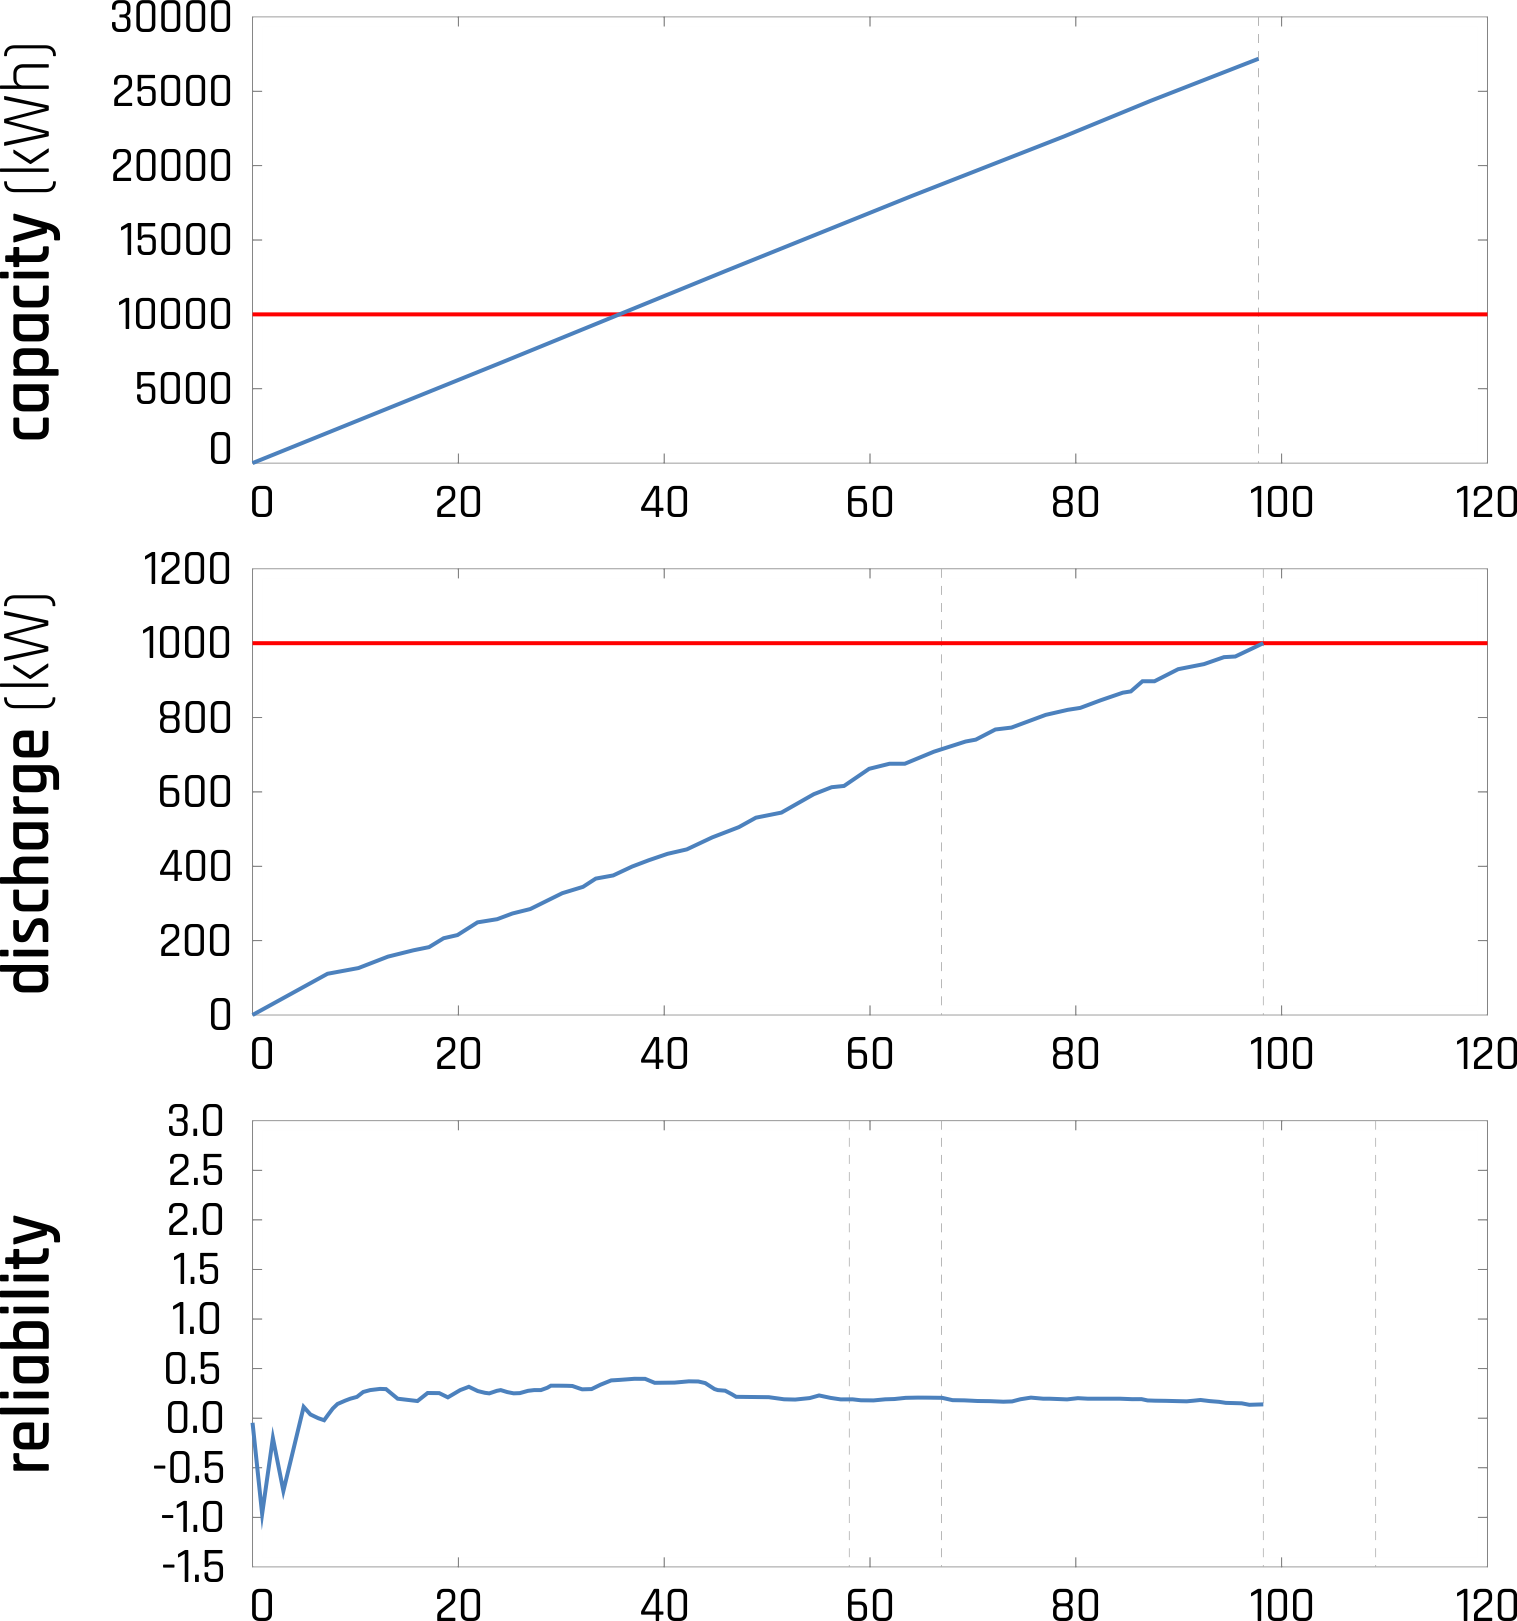
\includegraphics[scale=0.3]{clustering.png}
		\caption{Coalition formation with the\newline Clustering Algorithm\label{fig:clusteringcoalcreate}}
	\end{minipage}
\end{figure}
\vspace{-10pt}
Moreover, coalitions with fewer vehicles are preferable, since intuitively, this allows for a more efficient allocation of resources, and also means that fewer EVs will share the payoff associated with forming the coalition (exactly how this payoff allocation will occur, is a problem we do not deal with in this paper).
%On the figures~\ref{fig:samplecoalcreate}-~\ref{fig:transversalcoalcreate} the following is displayed:

To begin, in all Figs.~\ref{fig:heuristiccoalcreate}---\ref{fig:samplecoalcreate}:
\begin{itemize}
	\item In all subfigures, the horizontal axis depicts the progression of the coalition size.
	\item {\em Capacity subfig.} On the first graph of each figure, the capacity of the coalition is displayed. We can see how it is increased by selecting the appropriate agents until the goal (horizontal line) is reached.
	\item {\em Reliability subfig.} The second graph displays the mean reliability of our coalition.
	\item {\em Discharge subfig.} The third and last graph displays the discharge rate of the coalition. The goal of $1,000$ kW is shown as a horizontal line.
\end{itemize}
%As mentioned above, the lower the average completion time and the lower average coalition, the better. 
\paragraph{Heuristic Algorithm}
As explained in Section~\ref{sec:heuristic}, this algorithm attempts (in a rather ``greedy'' manner) to identify the best EVs from the hypergraph.	As we can observe in Fig.~\ref{fig:heuristiccoalcreate}, it takes on average only $58.5$ vehicles to reach the goal requirements, which is the most efficient use of resources observed across all our methods. The reliability achieved is also high, reaching a value of more than $1.5$. We remind the reader that the mean reliability of our pool of EVs is $0$. This approach is also the most time and memory efficient of all. Specifically the algorithms average completion time is only $25ms$ for these experiments, and it also scales linearly into the millions as seen in Fig.~\ref{fig:heuristicscaling} below.	
\paragraph{Clustering Algorithm}
This method performs clustering, as explained in Section~\ref{sec:Clustering}, and then takes random samples from the best cluster. Fig.~\ref{fig:clusteringcoalcreate} depicts its performance when using $k=3$ clusters. Unfortunately, we cannot control how exactly the clusters are formed, so we do not have a guarantee that high quality vehicles will be clustered together. This leads to a mediocre result with an increased average coalition size, and a slightly-over-the-average reliability. The average size of coalitions meeting both requirements is $98$. The average time required for the method's completion is $709 ms$. In Section~\ref{sec:results_modifications}, we show how different $k$ values affect our results.
\vspace{-10pt}
\begin{figure}
	\centering
	\begin{minipage}{.5\textwidth}
		\centering
		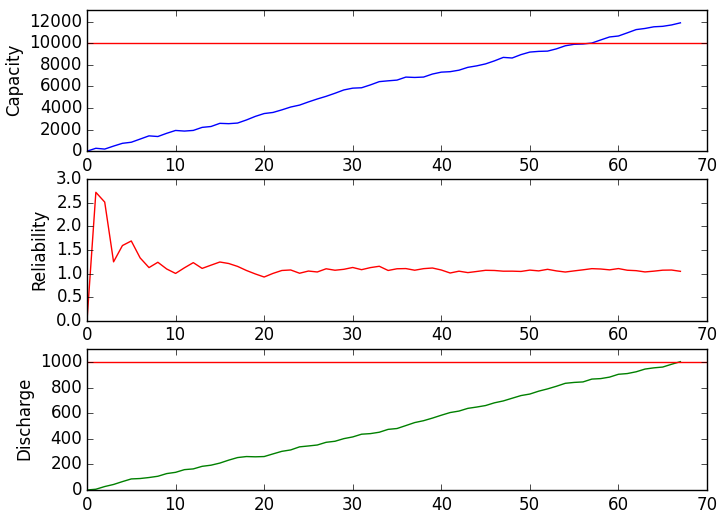
\includegraphics[scale=0.3]{transversal.png}
		\caption{Coalition formation with the\newline
			Minimal Transversal Algorithm \label{fig:transversalcoalcreate}}
	\end{minipage}%
	\begin{minipage}{.5\textwidth}
		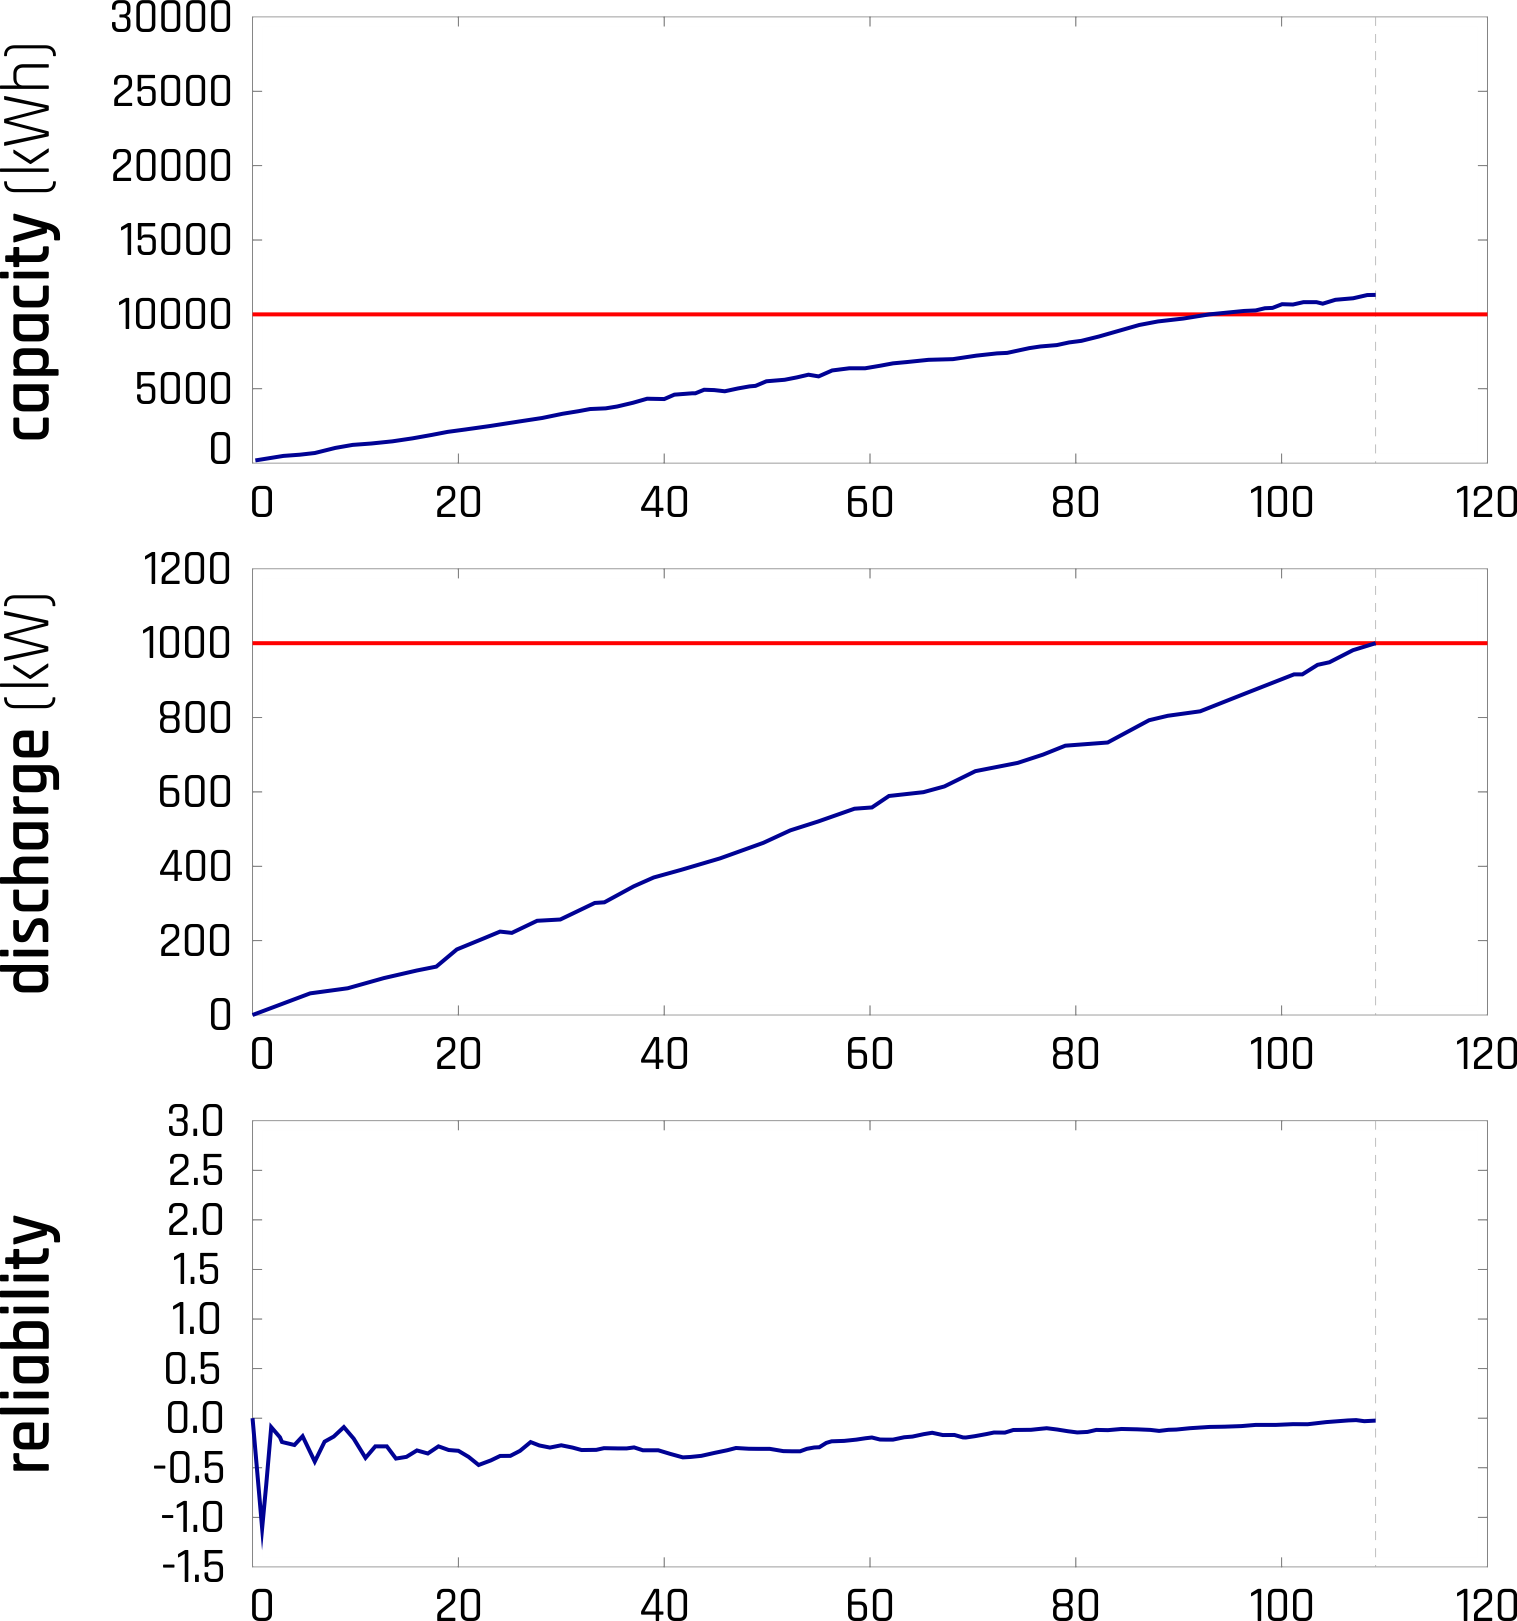
\includegraphics[scale=0.3]{sample.png}
		\caption{Coalition creation with the\newline
			Simple Sampling Algorithm \label{fig:samplecoalcreate}}
	\end{minipage}
\end{figure}
\vspace{-20pt}
\paragraph{Transversal}	
Using the transversal algorithm and taking nodes from a list of minimal hitting set. Fig.~\ref{fig:transversalcoalcreate} shows its performance. The transversal algorithm appears to work quite well since the average coalition size is only 64, slightly higher than that achieved by the heuristic approach. The reliability of the coalition is high, reaching  values over $1.1$. It can also scale quite well, reaching thousands of vehicles (cf. Fig.~\ref{fig:popscale}), but not as well as the heuristic approach. The average time to completion was $120ms$. %only.
\paragraph{Simple Sampling}
%Taking random samples until the set capacity and discharge goals, are achieved. 
Fig.~\ref{fig:samplecoalcreate} depicts our results for the Simple Sampling method. The average coalition size achieved with this algorithm is 109.3. The average completion time was 24ms. As expected, this algorithm achieves the weakest results among all our algorithms. The algorithms' performance is summarized in Table~\ref{tab:resultssum} for convenience.


\begin{table}
	\begin{center}
		\begin{tabular}{| c || c | c | c | c | }
			\hline
			Algorithm  & Heuristic & Clustering & Transversal & Simple Sampling\\ \hline
			Mean Coalition Size (\# EVs) & 58.5 & 98 & 64 & 109.3\\ \hline
			Mean Running Time ($ms$)  & 25 & 709 & 120 & 24\\ \hline
			Mean Generat.+Run. Time  ($ms$)  &  1041 & 1725  & 1136 & 1040\\ \hline
		\end{tabular}
	\end{center}
	
	\caption{Summarizing the performance results\label{tab:resultssum}}
\end{table}	
\vspace{-20pt}
\subsection{Scaling Behaviour}
We now test the scaling behaviour of our algorithms. First, we show how our algorithms scale with time when the \textit{capacity} goal is increased. Then, we show how they scale as the number of EVs  under consideration increases.

%	\begin{table}
%		\begin{center}
%			\begin{tabular}{| c || c | c | c | }
%				\hline
%				Goal (kWh)& Heuristic (sec) & Clustering (sec) & Transversal (sec) \\ \hline
%				10,000  & 0.03& 0.049 & 0.20\\ \hline
%				40,000  & 0.04 & 0.049 & 0.36  \\ \hline
%				70,000  & 0.06 & 0.049 & 0.34  \\ \hline
%				100,000 & 0.11 & 0.049 & 0.33 \\ \hline
%				130,000 & 0.19 & 0.049 & 0.33  \\ \hline
%				160,000 & 0.28 & 0.049 & 0.33  \\ \hline
%				190,000 & 0.39 & 0.049 & 0.34  \\ \hline
%				220,000 & 0.50 & 0.049 & 0.32  \\ \hline
%				250,000 & 0.64 & 0.049 & 0.32  \\ \hline
%				280,000 & 0.86 & 0.049 & 0.32  \\ \hline
%			\end{tabular}
%		\end{center}
%		\caption{Scaling against an increasing ``capacity'' goal\label{tab:goalscale}}
%	\end{table}

In Fig.~\ref{fig:goalscale} %and Table~\ref{tab:goalscale} 
we can see how the transversal, heuristic and clustering algorithm scale against an increasing capacity goal (assuming any other goal remains fixed). The starting size of the available agents was kept constant at $20,000$ EVs for this experiment. We observe that the scaling behaviour of the heuristic algorithm against an increasing capacity goal is exponential. %  in execution time. 
Nevertheless, its total required execution time is low, since it takes the algorithm 0.9 seconds to reach the goal capacity of 300,000 $kWh$.
\begin{figure}
	\centering
	\begin{minipage}{.5\textwidth}
		\centering
		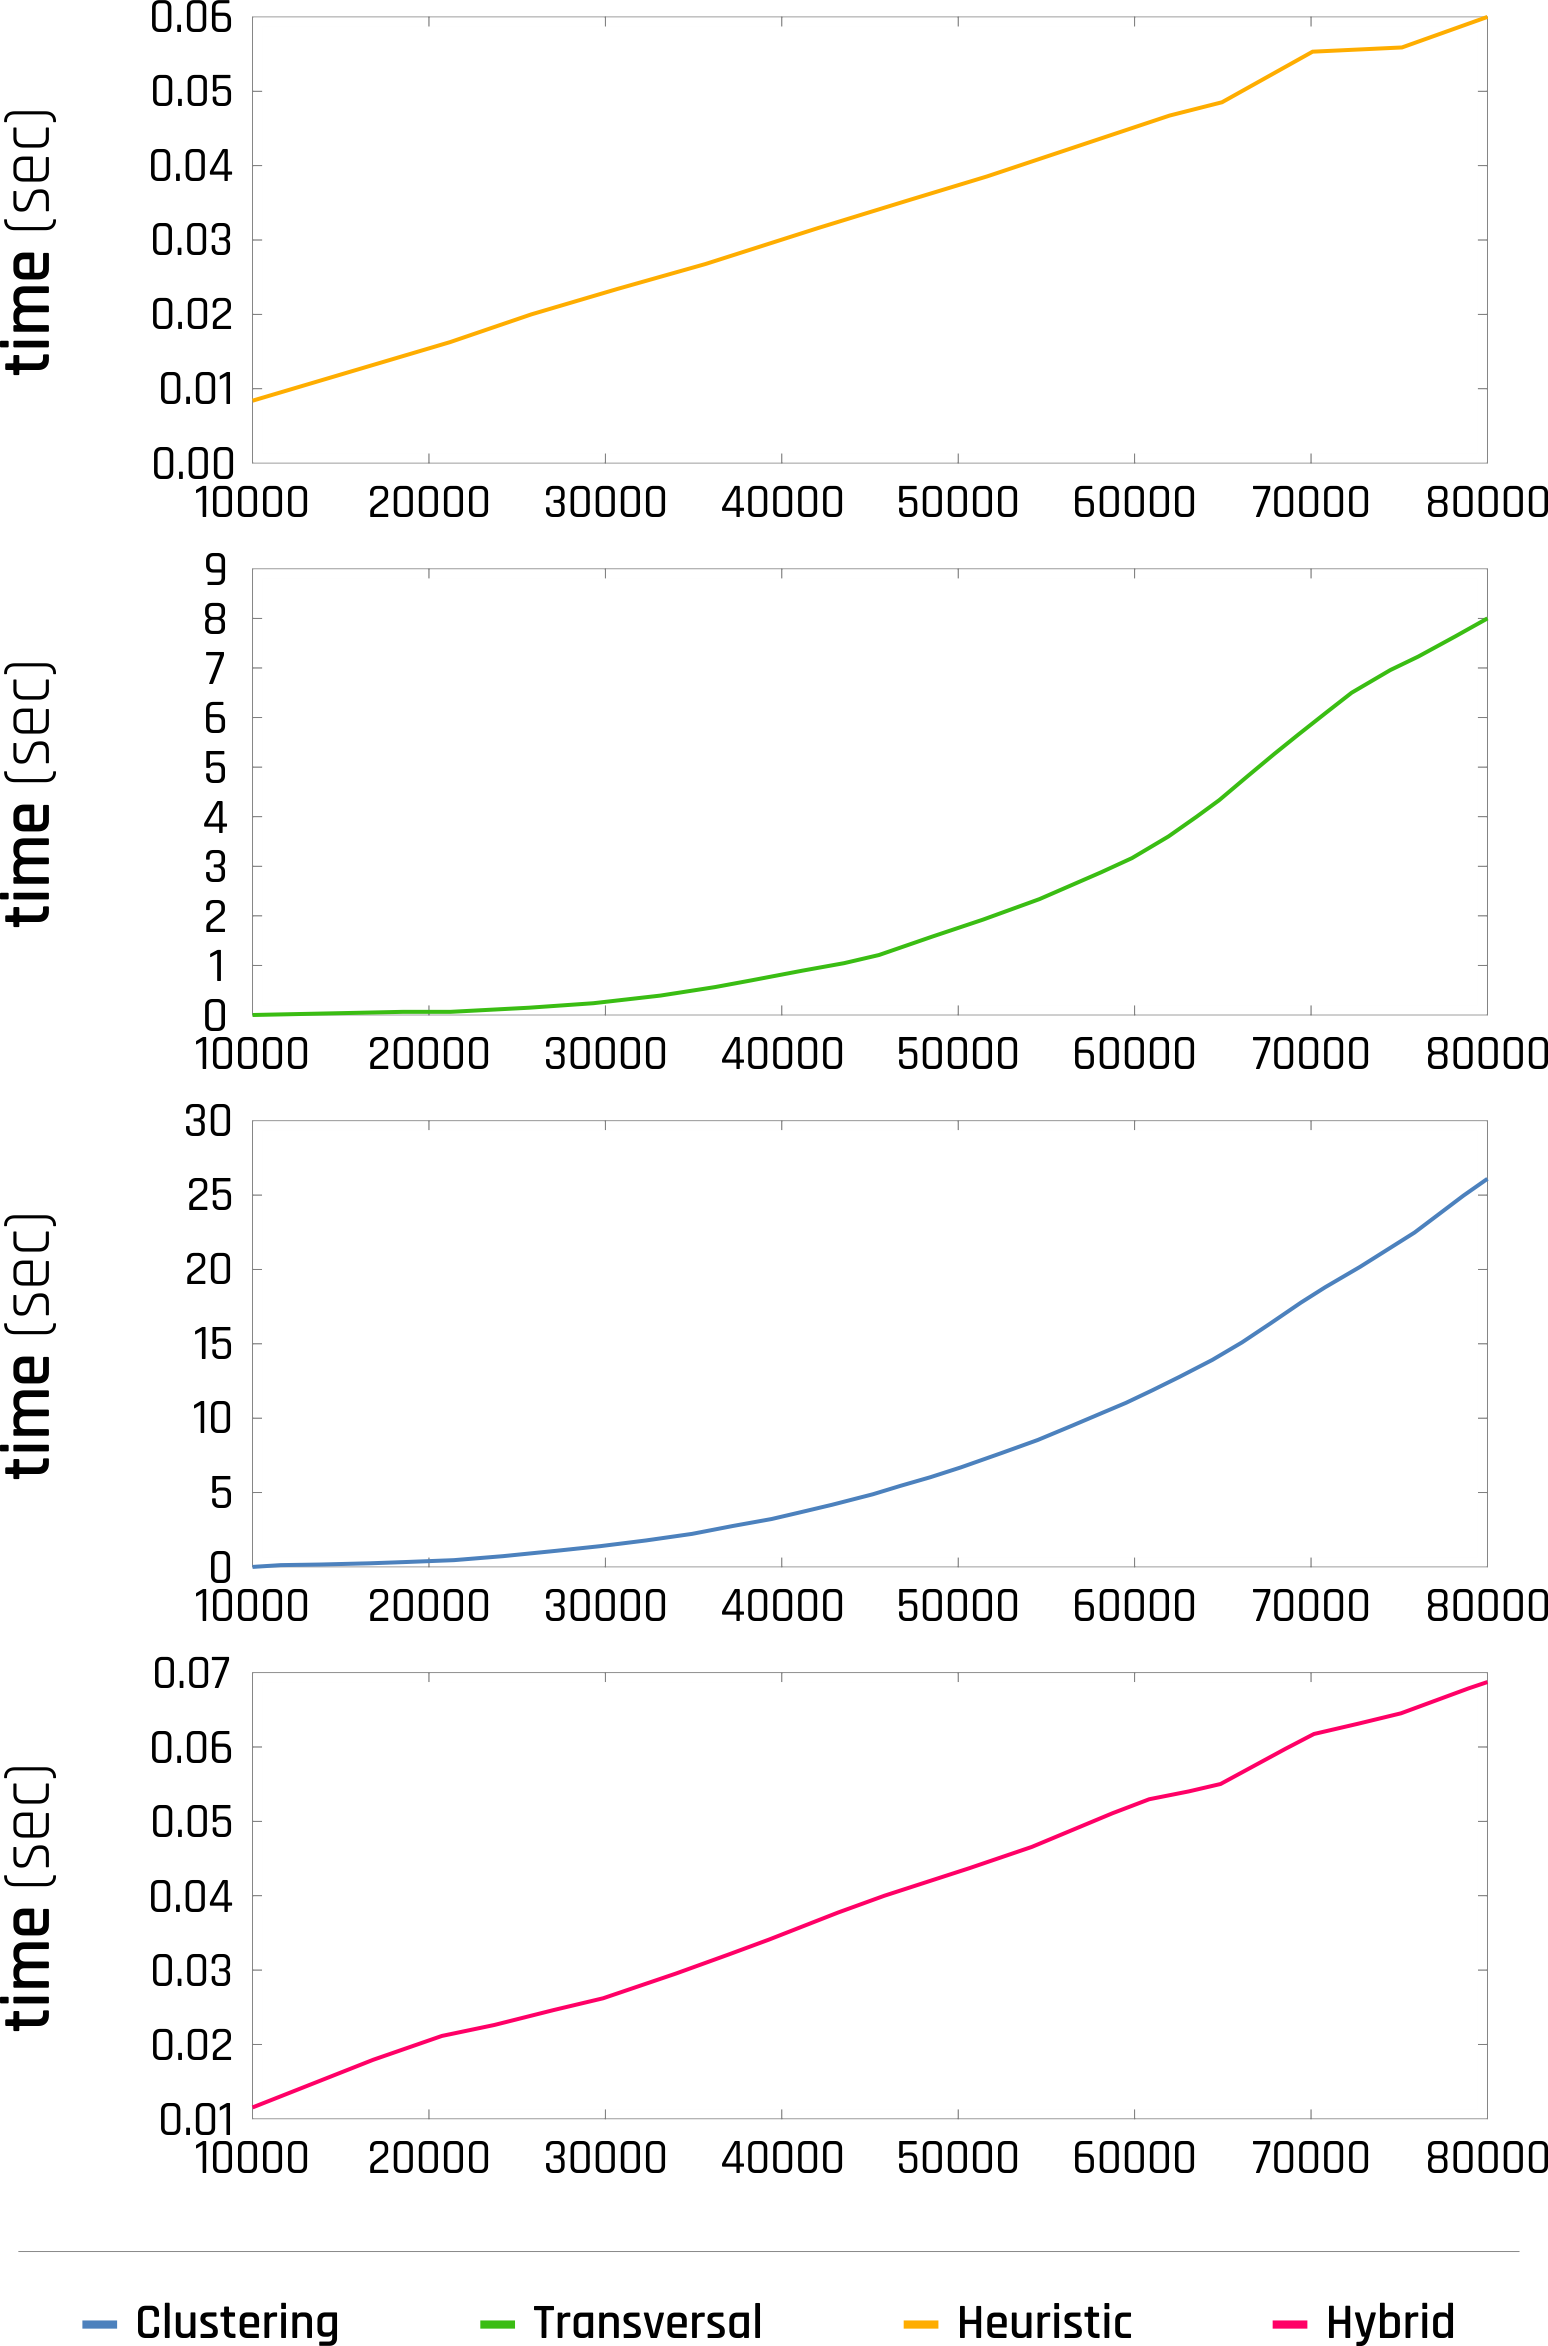
\includegraphics[scale=0.3]{node_scaling.png}
		\caption{Scaling against an increasing
			\newline EV population\label{fig:popscale}}
	\end{minipage}%
	\begin{minipage}{.5\textwidth}
		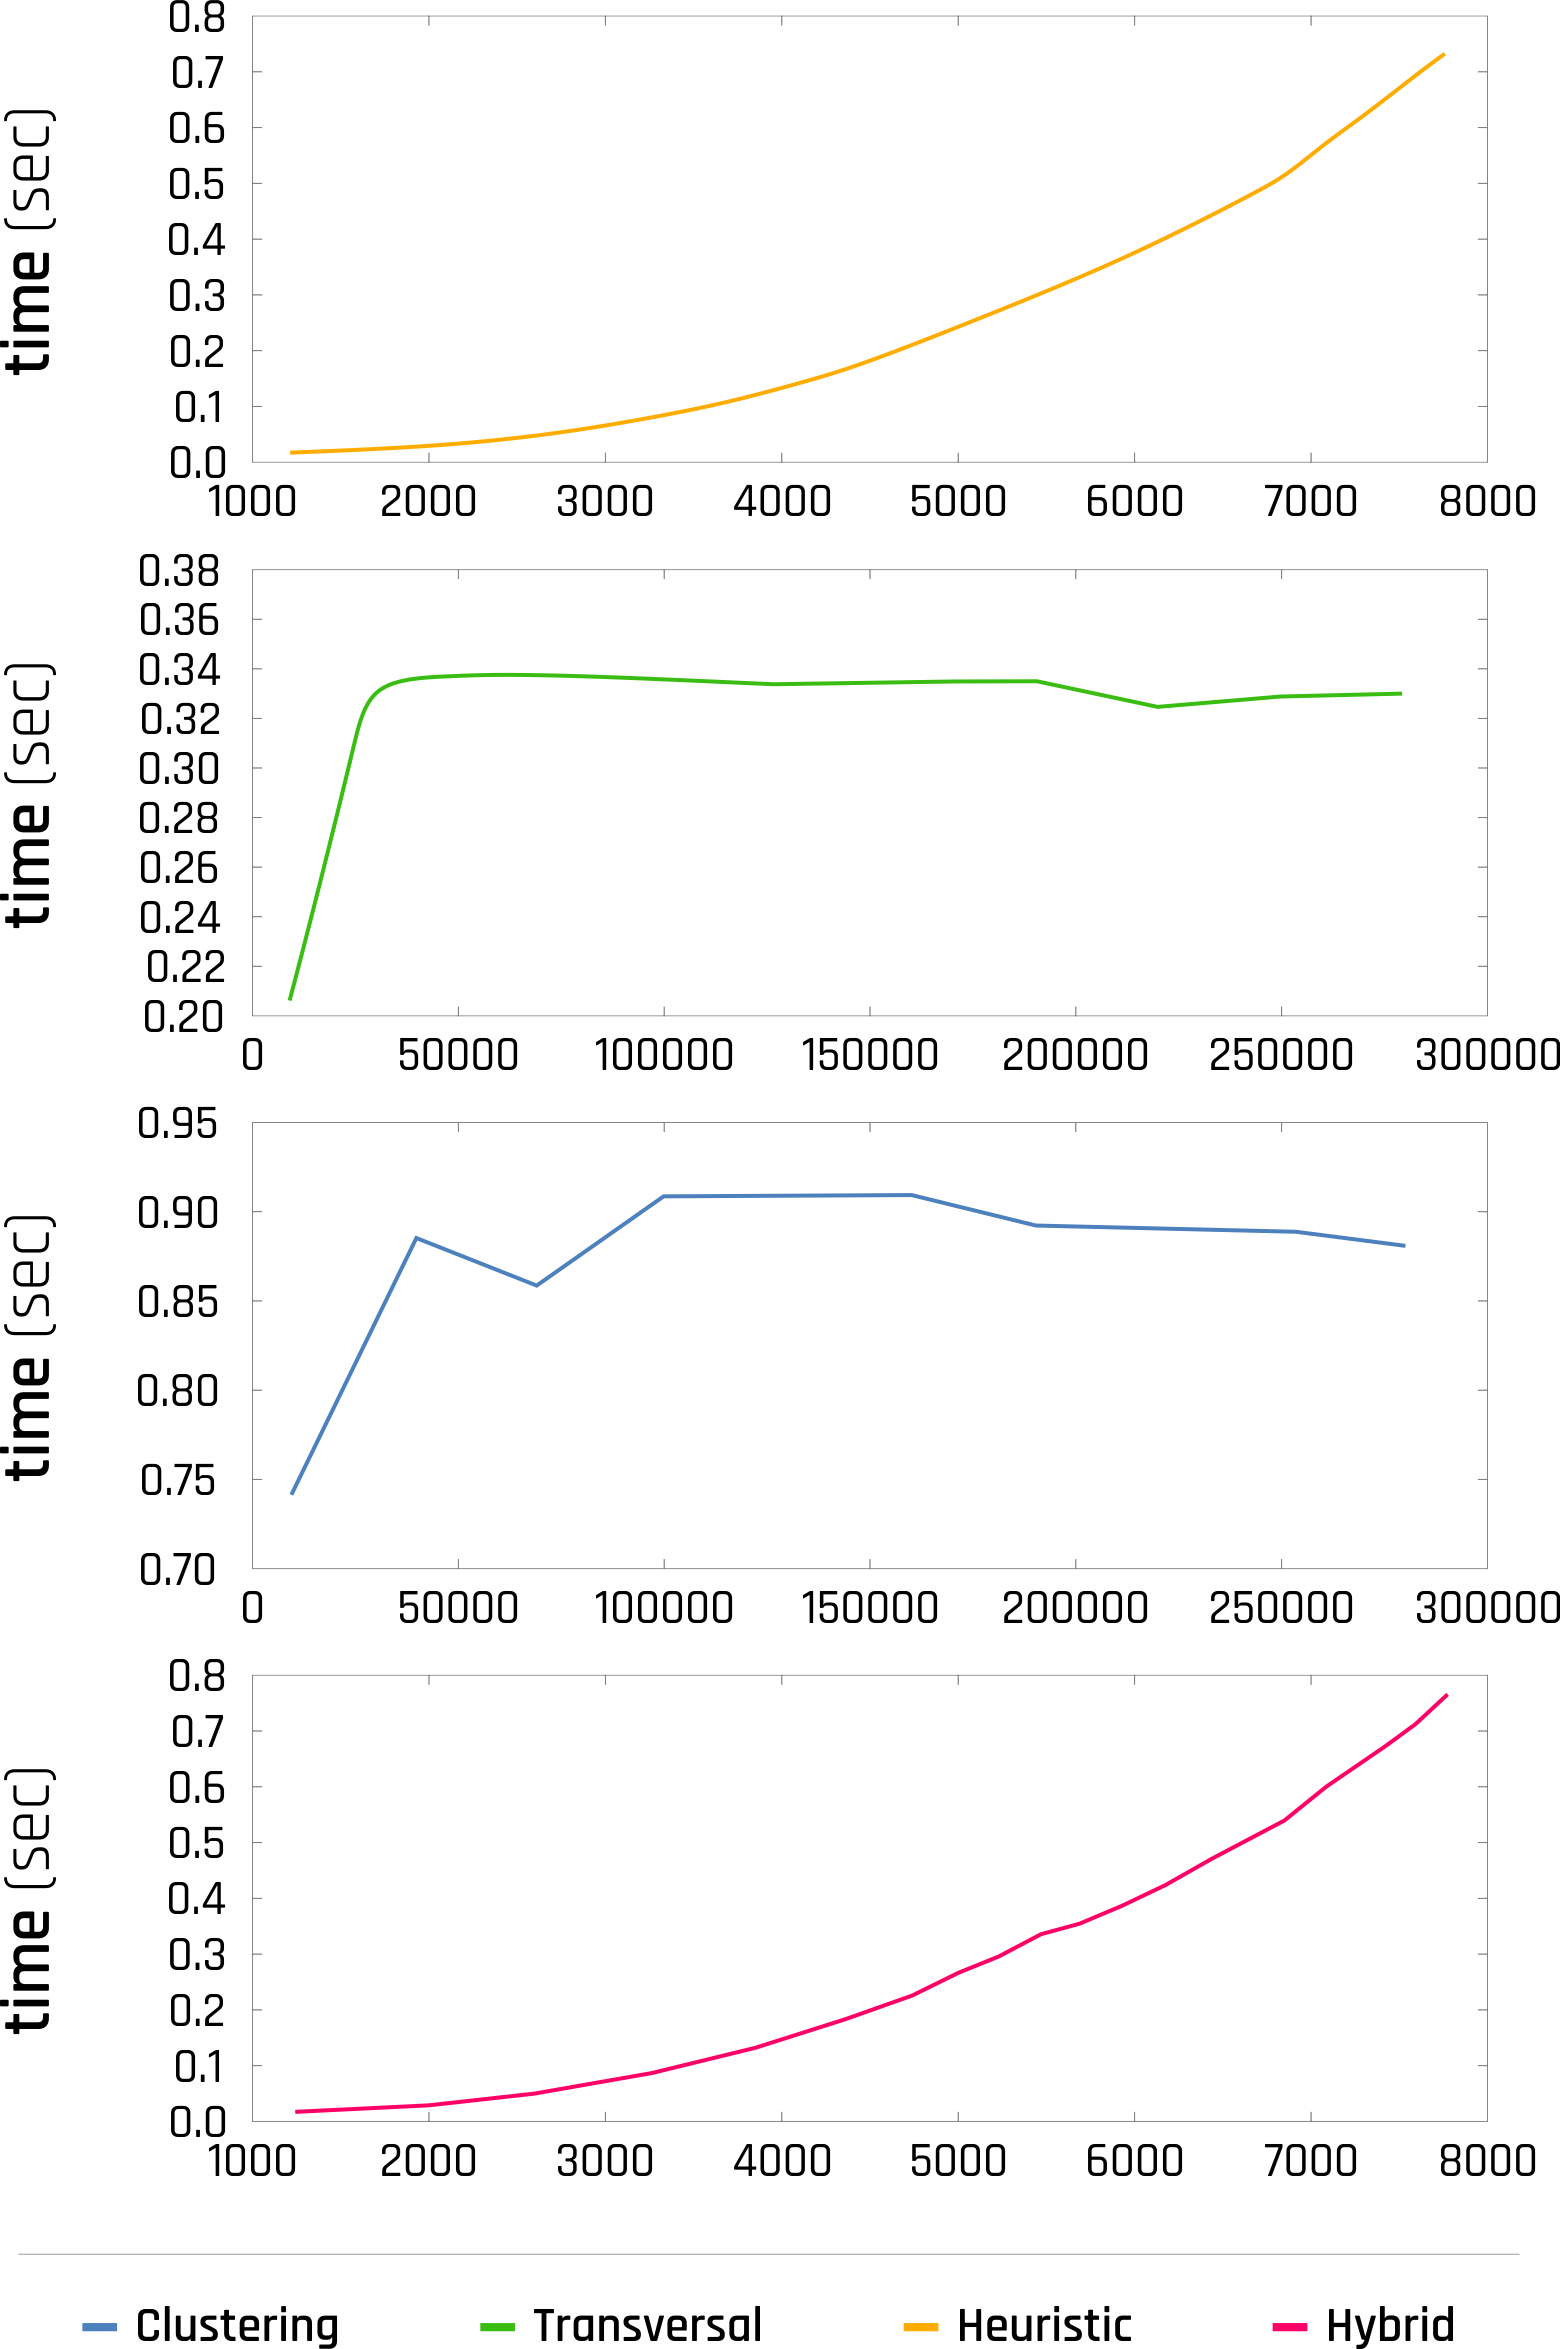
\includegraphics[scale=0.3]{goal_scaling.png}
		\caption{Scaling against an increasing\newline ``capacity'' goal\label{fig:goalscale}}
	\end{minipage}
\end{figure}
\vspace{-10pt}
The transversal algorithm scales with steps. The main reason for this is that the minimal transversal sets are generated before we select the agents of a coalition. If a minimal transversal set does not achieve the goal capacity, we generate a new one with more agents, till we reach the set capacity goal. This generates a step pattern, the first stages of which are shown in Fig.~\ref{fig:goalscale}. In Fig.~\ref{fig:goalscale} we actually manage to see only one step because generating the minimal transversals with $3$ EVs is enough to find good coalitions for all goals from $40,000$ $kWh$ onwards (while it was enough to generate the minimal transversals with $2$ EVs to cover the $10,000$ $kWh$ capacity goal). %Note that though it takes the transversal algorithm more than twice the time of the heuristic to scale to 300MWh, this time, is still low ($<30$sec).  
%Finally, the clustering algorithm's running time is constant irrespective of increase in the capacity goal. 
%The reason for this is that clustering, which is the part of the algorithm that requires the most processing power, takes place regardless of the final coalition requirements.
%In conclusion, the transversal algorithm exhibits the worst scaling behaviour against an increasing capacity goal, while the clustering algorithm's running time is not influenced by such an increase. 

Now, the running time of the hypegraph clustering algorithm is largely independent of the size of the stated capacity goal. 
This is because the clustering itself, which is the part of the algorithm that requires the most processing power, takes place regardless of the final coalition requirements.
Indeed, we observe in Fig.~\ref{fig:goalscale} that after an initial jump due to increased sampling requirements (cf. lines 6---8, Alg.~\ref{alg:clustering}) when moving from a goal of $10,000$ to $40,000$ $kWh$,
the algorithm's running time remains largely unaltered.


Fig.~\ref{fig:popscale} %and table~\ref{tab:popscale} 
displays scaling against the initial EV population. The coalition goals were kept constant, and the same for all algorithms.
The heuristic algorithm shows a linear scaling in time as the agent size grows. Specifically, the heuristic algorithm can scale {\em up to a million agents} within an acceptable time. 


Fig.~\ref{fig:heuristicscaling} demonstrates this behaviour, starting from $50,000$ EVs. Of course, one expects that when the population reaches several millions, the complexity of the sorting algorithm will kick in, creating bottlenecks. Regardless, the fact that linear scalability is maintained up to $1,000,000$ agents is reassuring. By contrast, looking at Fig.~\ref{fig:popscale}, we observe that the transversal and clustering algorithms scale exponentially.

\begin{figure}
	\centering
	\begin{minipage}{.5\textwidth}
		\centering
		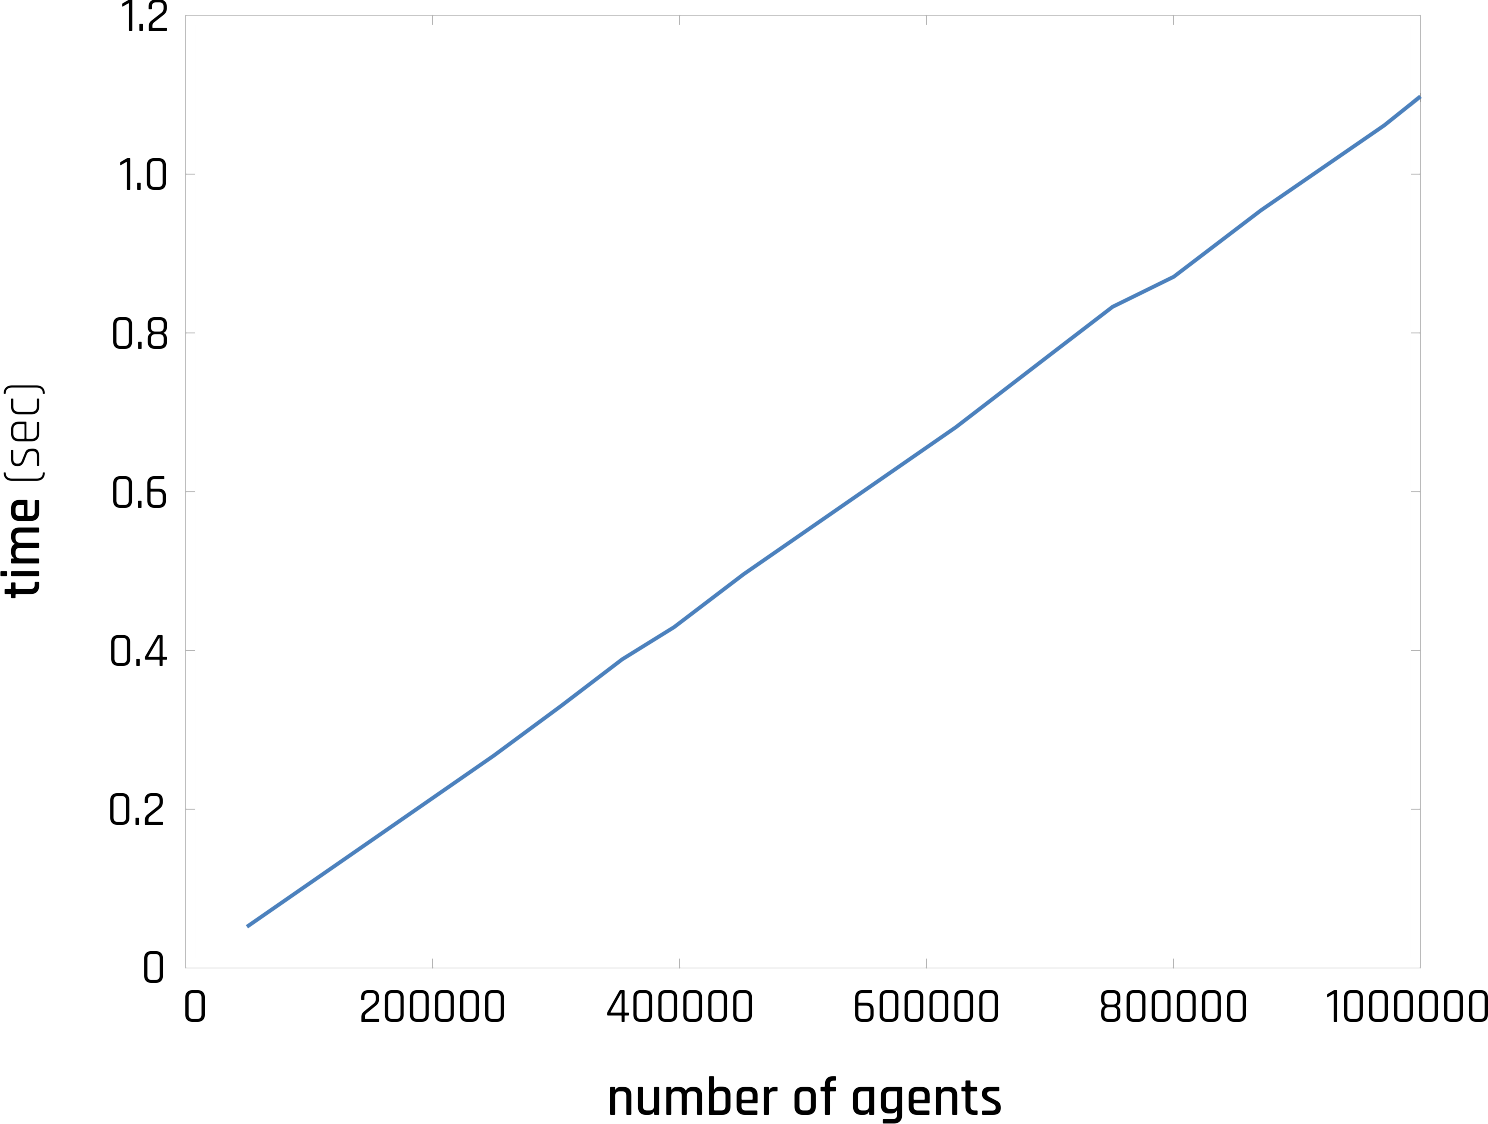
\includegraphics[scale=0.3]{greedy_node_scaling.png}
		
		\caption{Scaling of the Heuristic Algorithm\label{fig:heuristicscaling}}
		\vspace{20pt}
	\end{minipage}%
	\begin{minipage}{.5\textwidth}
		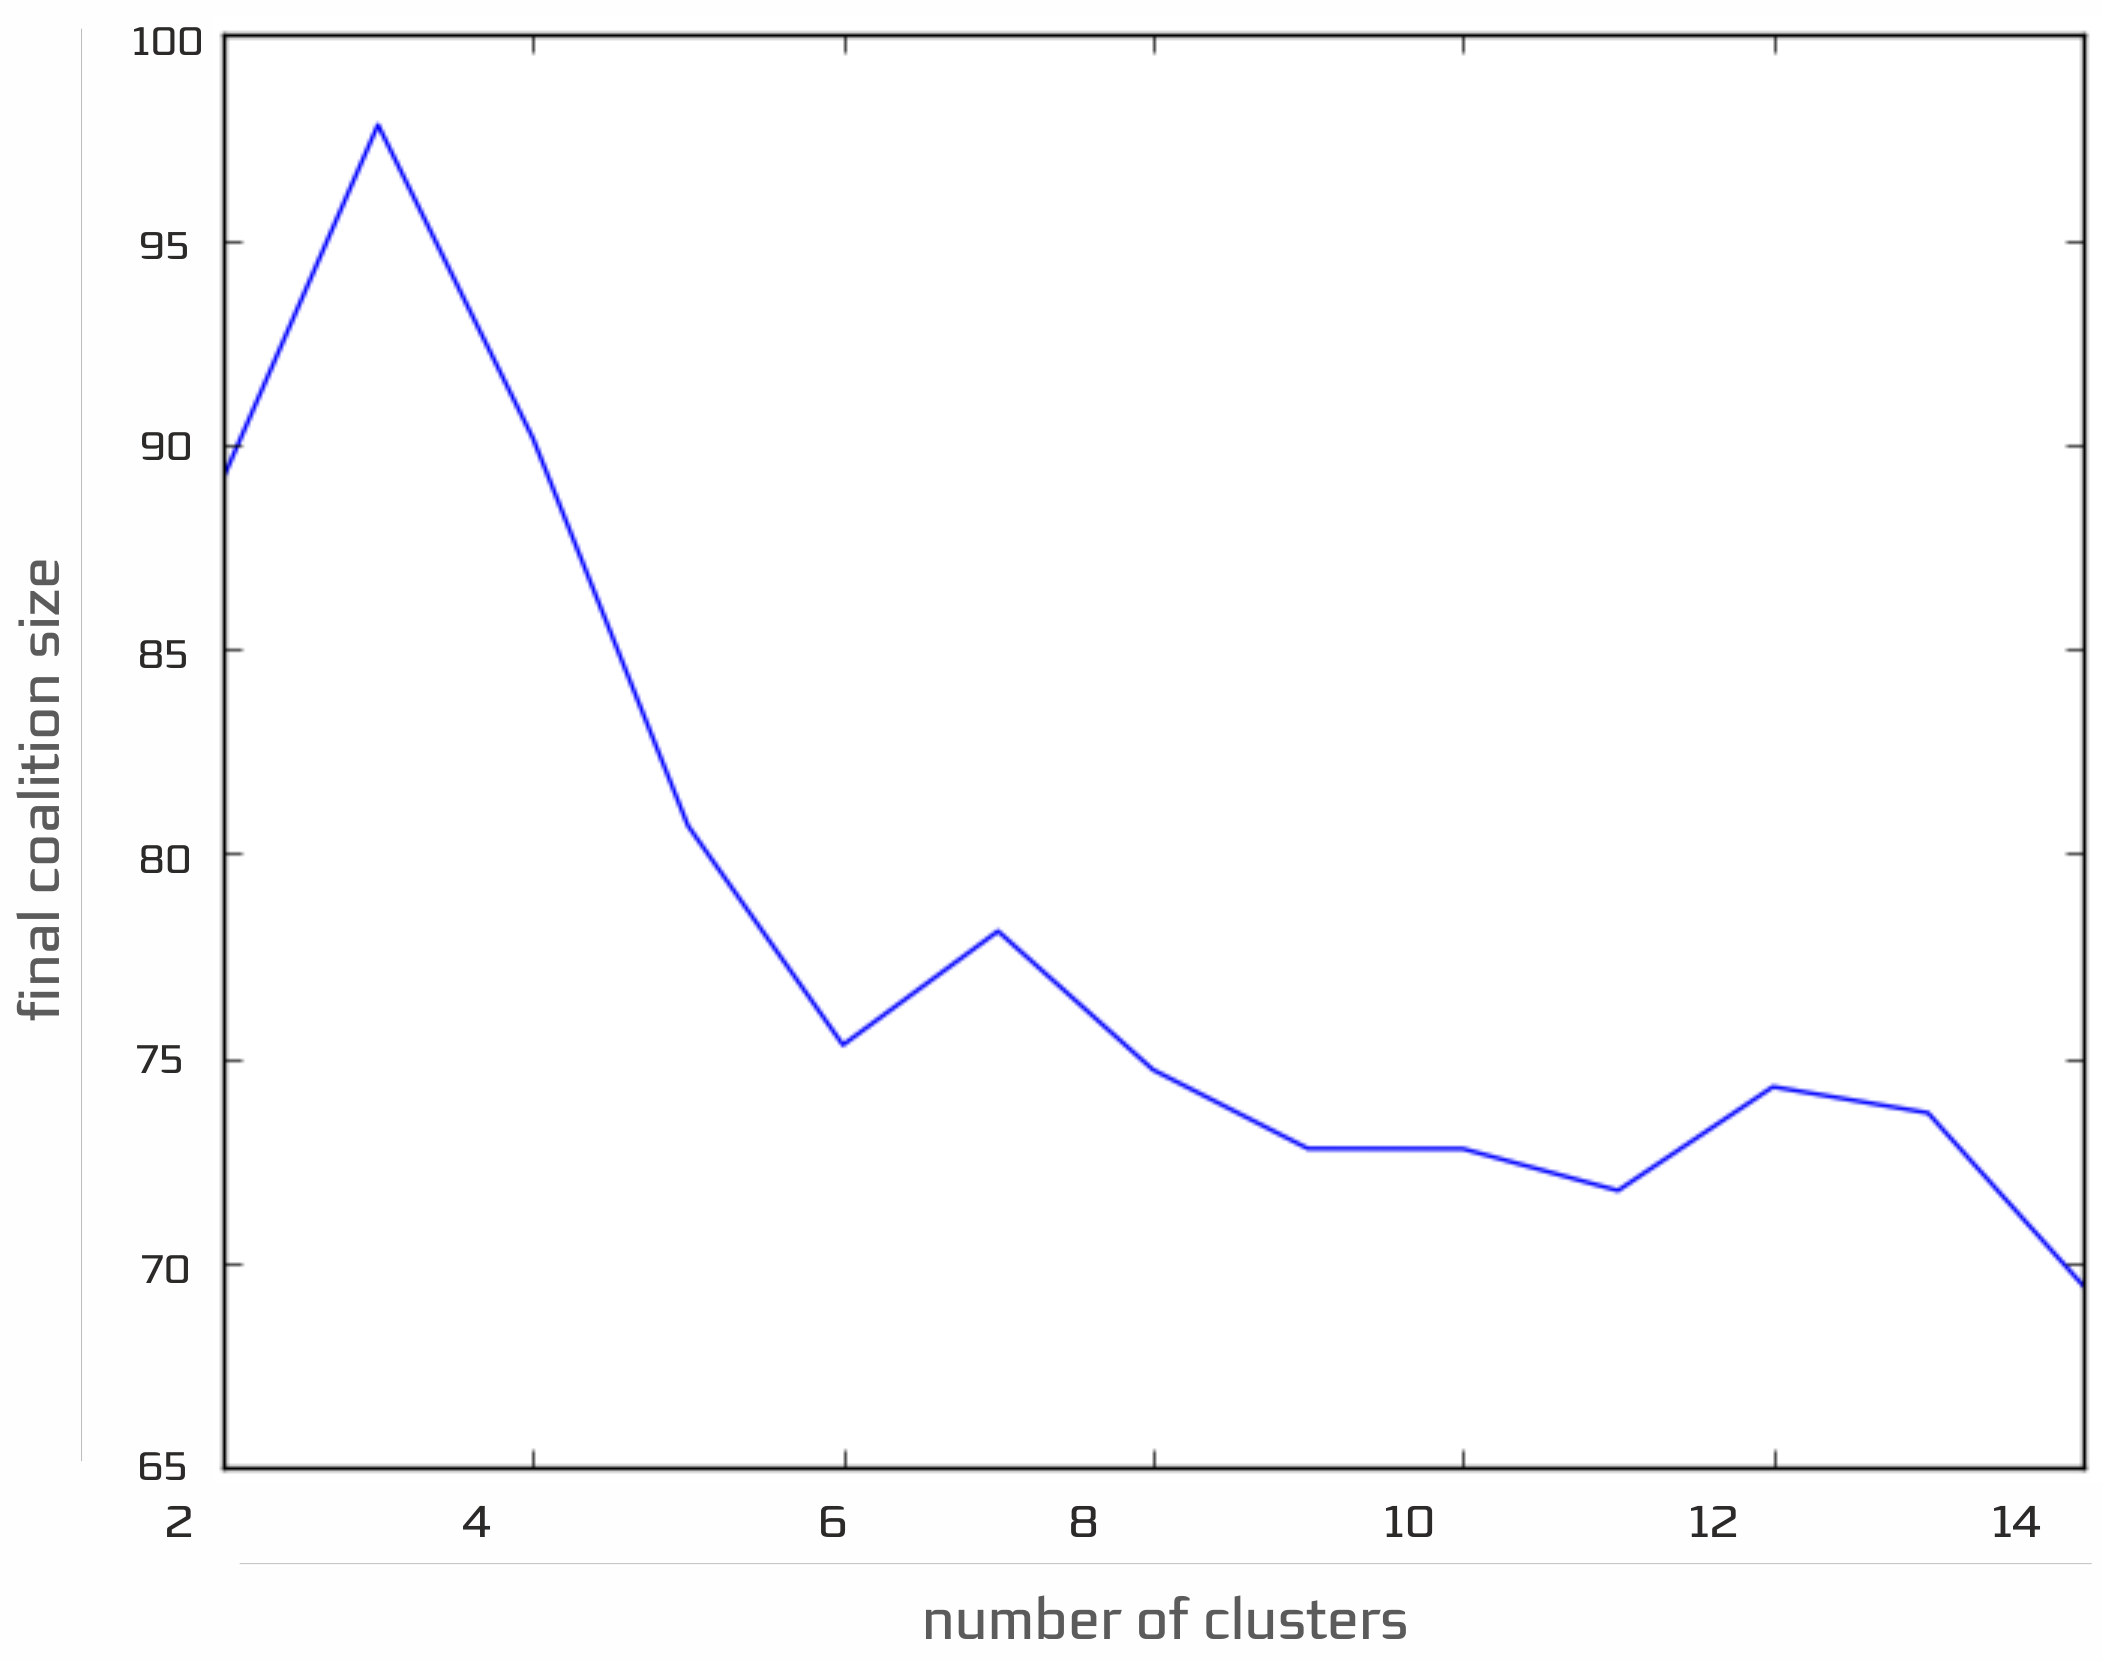
\includegraphics[scale=0.3]{number_of_clusters.png}
		\caption{Evolution of the average size of coalitions produced with the Hypergraph Clustering method, when varying the number of clusters\label{fig:clusterkscale}}
	\end{minipage}
\end{figure}
\vspace{-30pt}

%	\begin{table}		
%		\begin{center}
%			\begin{tabular}{| c || c | c | c | }
%				\hline
%				EVs   & Heuristic (sec) & Clustering (sec) & Transversal (sec) \\ \hline
%				10,000 & 0.012 & 0.14 & 0.03  \\ \hline
%				11,000 & 0.013 & 0.17 & 0.04\\ \hline
%				12,000 & 0.015 & 0.22 & 0.05\\ \hline
%				13,000 & 0.016 & 0.25 & 0.06  \\ \hline
%				14,000 & 0.017 & 0.31 & 0.07\\ \hline
%				15,000 & 0.018 & 0.11 & 0.07\\ \hline
%				16,000 & 0.019 & 0.36 & 0.08 \\ \hline
%				17,000 & 0.020 & 0.43 & 0.08\\ \hline
%				18,000 & 0.021 & 0.50 & 0.09 \\ \hline
%				19,000 & 0.023 & 0.57 & 0.10  \\ \hline
%				20,000 & 0.024 & 0.69 & 0.12\\ \hline
%			\end{tabular}
%		\end{center}
%		\caption{Scaling against an increasing EV population\label{tab:popscale}}
%	\end{table}

\subsection{Varying the number of hypergraph clusters} \label{sec:results_modifications}
We test our clustering algorithm further by modifying the number of clusters, $k$, since this is a parameter that can be optimized empirically, as explained in Section~\ref{sec:Clustering}.

Fig.~\ref{fig:clusterkscale} displays the relation between \textit{k} and the average coalition size that results from the clustering method (and which achieves the set goals). Creating a larger number of clusters results in smaller, and thus better, coalitions. Regardless, even when $k=15$, the clustering algorithm still produces coalitions with more EVs than the heuristic one.% ($69$ compared to $58.5$).
 
%\include{Chapters/Chapter5} 

%----------------------------------------------------------------------------------------
%	THESIS CONTENT - APPENDICES
%----------------------------------------------------------------------------------------

\appendix % Cue to tell LaTeX that the following "chapters" are Appendices

% Include the appendices of the thesis as separate files from the Appendices folder
% Uncomment the lines as you write the Appendices

% Appendix A

\chapter{Appendix Title Here} % Main appendix title

\label{AppendixA} % For referencing this appendix elsewhere, use \ref{AppendixA}

Write your Appendix content here.
%\include{Appendices/AppendixB}
%\include{Appendices/AppendixC}

%----------------------------------------------------------------------------------------
%	BIBLIOGRAPHY
%----------------------------------------------------------------------------------------

\printbibliography[heading=bibintoc]

%----------------------------------------------------------------------------------------

\end{document}  
